\chapter{RESULTS AND ANALYSIS}

\section{Comparative Analysis of Object Detection using YOLOv5 and YOLOv7}

\subsection{Experimental Setup}

A comparative study using \gls{yolo}v5 and \gls{yolo}v7 to detect and classify hand-drawn electronic circuit components was conducted to determine which model is better-suited for the needs of this project. The dataset consisted of 61 classes, including resistors, capacitors (polarized and unpolarized), diodes, transistors (\gls{bjt} and \gls{fet}), integrated circuits, switches, and more. To ensure a fair comparison, both models were trained and validated on identical data splits.

\subsection{Performance Metrics}

\subsubsection{mAP vs Number of Epochs}

In order to monitor the progress in models' ability to recognize components as the training progressed, \gls{map}@0.5 was plotted across all epochs. These curves depict how quickly and effectively each model learns over time.

\begin{figure}[htbp]
    \centering
    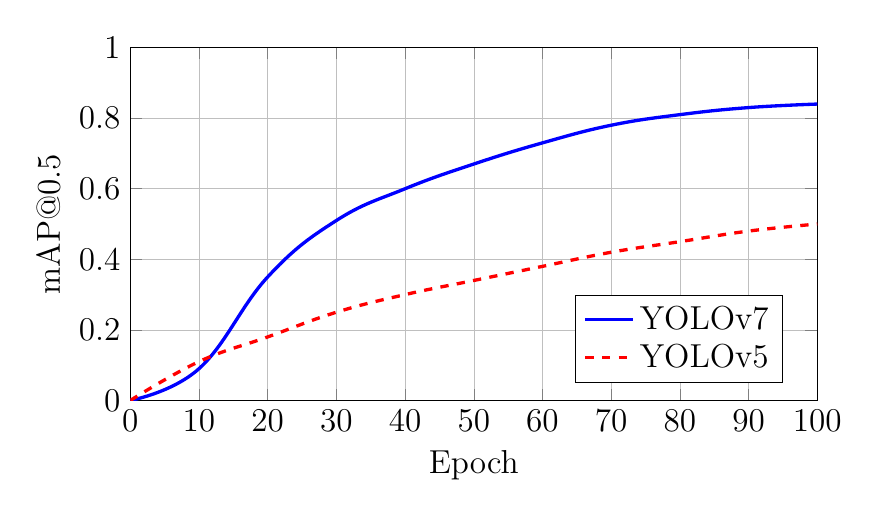
\begin{tikzpicture}
    \begin{axis}[
        width=0.85\textwidth,
        height=0.5\textwidth,
        xlabel={Epoch},
        ylabel={mAP@0.5},
        xmin=0, xmax=100,
        ymin=0, ymax=1,
        grid=both,
        major grid style={line width=.2pt, draw=gray!50},
        tick label style={font=\large},
        label style={font=\large},
        legend style={at={(0.95,0.05)}, anchor=south east, font=\large}
    ]
    \addplot[smooth, tension=0.7, blue, very thick] coordinates {
        (0,0.00) (10,0.09) (20,0.35) (30,0.51) (40,0.60)
        (50,0.67) (60,0.73) (70,0.78) (80,0.81) (90,0.83) (100,0.84)
    };
    \addlegendentry{YOLOv7}
    \addplot[smooth, tension=0.7, red, dashed, very thick] coordinates {
        (0,0.00) (10,0.11) (20,0.18) (30,0.25) (40,0.30)
        (50,0.34) (60,0.38) (70,0.42) (80,0.45) (90,0.48) (100,0.50)
    };
    \addlegendentry{YOLOv5}
    \end{axis}
    \end{tikzpicture}
    \caption{mAP@0.5 comparison over 100 training epochs.}
    \label{fig:map_epochs}
\end{figure}

It is clear from \cref{fig:map_epochs} that the \gls{map} score for \gls{yolo}v7 are significantly better than that for \gls{yolo}v5.

\subsubsection{Precision vs Recall and F1 Score vs Confidence}

\begin{figure}[htbp]
    \centering
    \begin{minipage}[t]{0.48\textwidth}
        \centering
        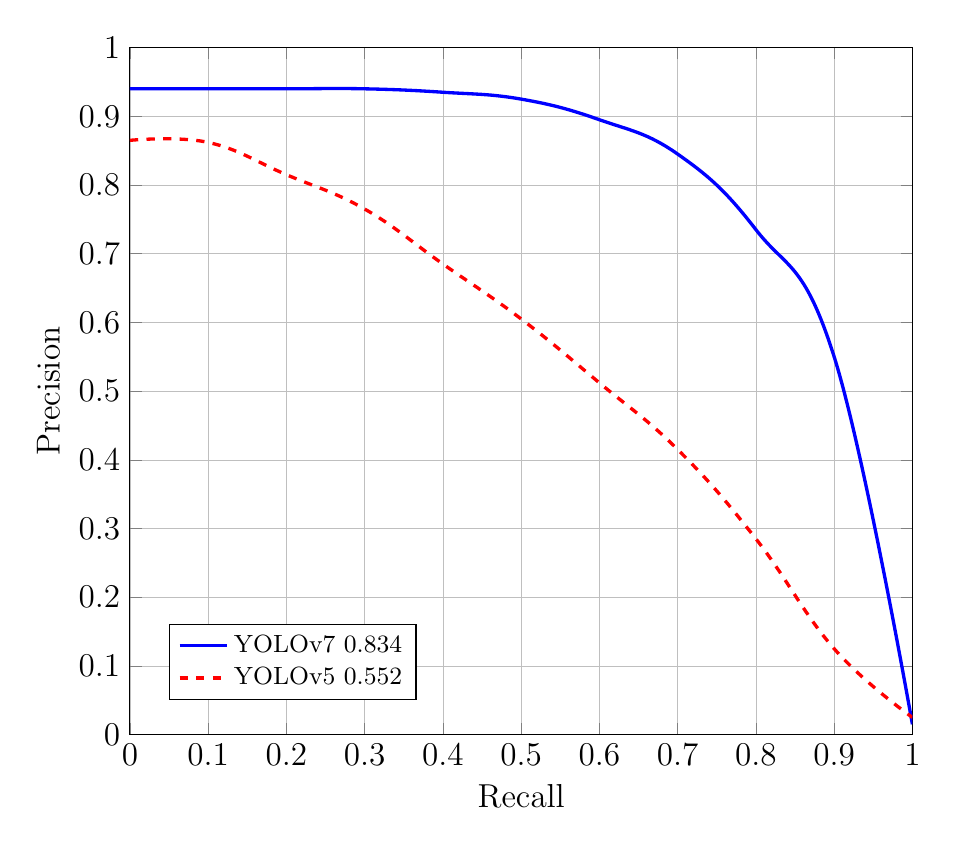
\begin{tikzpicture}
        \begin{axis}[
            width=0.95\textwidth,
            height=0.85\textwidth,
            xlabel={Recall},
            ylabel={Precision},
            xmin=0, xmax=1,
            ymin=0, ymax=1,
            grid=both,
            major grid style={line width=.2pt, draw=gray!50},
            tick label style={font=\large},
            label style={font=\large},
            legend style={at={(0.05,0.05)}, anchor=south west, font=\small}
        ]
        \addplot[smooth, tension=0.7, blue, very thick] coordinates {
            (0.000,0.940) (0.100,0.940) (0.200,0.940) (0.300,0.940)
            (0.400,0.935) (0.500,0.925) (0.600,0.895) (0.700,0.845)
            (0.800,0.735) (0.900,0.550) (1.000,0.015)
        };
        \addlegendentry{YOLOv7 0.834}
        \addplot[smooth, tension=0.7, red, dashed, very thick] coordinates {
            (0.000,0.865) (0.100,0.862) (0.200,0.815) (0.300,0.765)
            (0.400,0.685) (0.500,0.605) (0.600,0.512) (0.700,0.415)
            (0.800,0.285) (0.900,0.125) (1.000,0.025)
        };
        \addlegendentry{YOLOv5 0.552}
        \end{axis}
        \end{tikzpicture}
        \subcaption{Precision-Recall curve.}
        \label{fig:pr_curve}
    \end{minipage}
    \hfill
    \begin{minipage}[t]{0.48\textwidth}
        \centering
        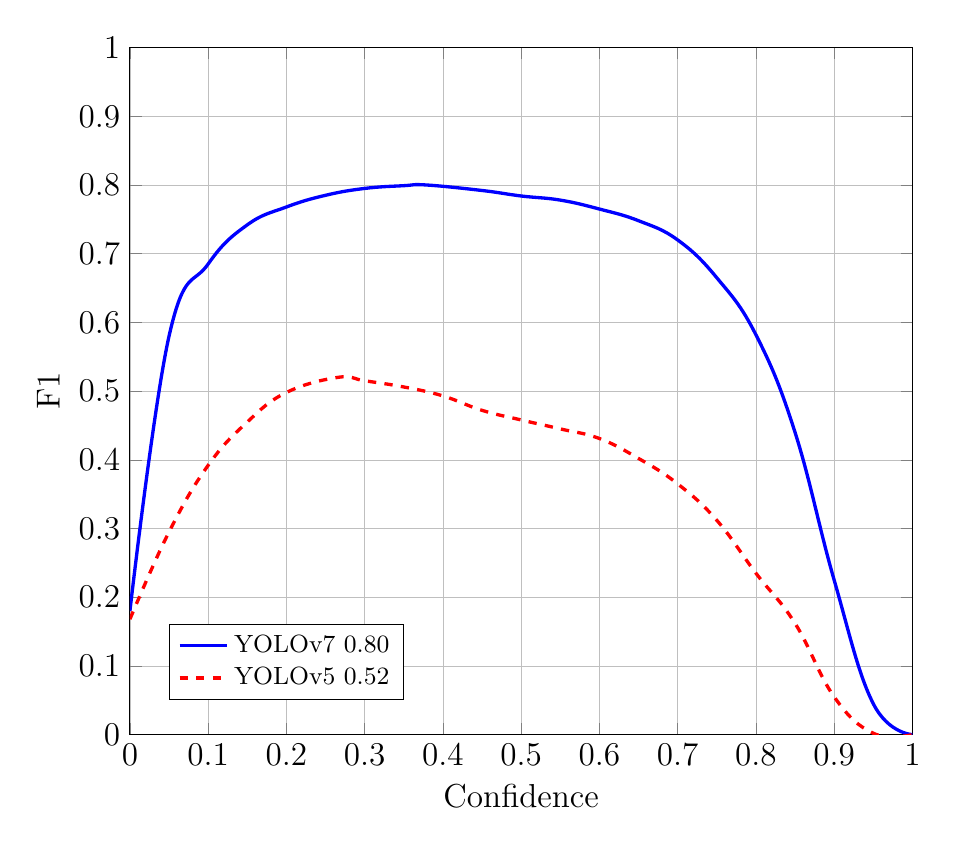
\begin{tikzpicture}
        \begin{axis}[
            width=0.95\textwidth,
            height=0.85\textwidth,
            xlabel={Confidence},
            ylabel={F1},
            xmin=0, xmax=1,
            ymin=0, ymax=1,
            grid=both,
            major grid style={line width=.2pt, draw=gray!50},
            tick label style={font=\large},
            label style={font=\large},
            legend style={at={(0.05,0.05)}, anchor=south west, font=\small}
        ]
        \addplot[smooth, tension=0.7, blue, very thick] coordinates {
            (0.000,0.180) (0.050,0.580) (0.100,0.685) (0.150,0.742)
            (0.200,0.768) (0.250,0.785) (0.300,0.795) (0.350,0.799)
            (0.379,0.800) (0.450,0.792) (0.500,0.784) (0.550,0.778)
            (0.600,0.765) (0.650,0.748) (0.700,0.720) (0.750,0.665)
            (0.800,0.582) (0.850,0.440) (0.900,0.225) (0.950,0.045)
            (1.000,0.000)
        };
        \addlegendentry{YOLOv7 0.80}
        \addplot[smooth, tension=0.7, red, dashed, very thick] coordinates {
            (0.000,0.168) (0.050,0.295) (0.100,0.392) (0.150,0.455)
            (0.200,0.498) (0.266,0.520) (0.300,0.515) (0.350,0.506)
            (0.400,0.493) (0.450,0.472) (0.500,0.458) (0.550,0.445)
            (0.600,0.431) (0.650,0.402) (0.700,0.365) (0.750,0.312)
            (0.800,0.235) (0.850,0.162) (0.900,0.055) (0.950,0.002)
            (1.000,0.000)
        };
        \addlegendentry{YOLOv5 0.52}
        \end{axis}
        \end{tikzpicture}
        \subcaption{F1-Confidence curve.}
        \label{fig:f1_curve}
    \end{minipage}
    \caption{Performance metrics comparison: (a) Precision-Recall and (b) F1-Confidence curves.}
    \label{fig:performance_metrics}
\end{figure}

\cref{fig:performance_metrics} demonstrate the F1 Score-Confidence Curve for YOLOv5 and YOLOv7 respectively. The larger the area under this curve, the higher the robustness of the precision-recall trade-off across thresholds.

\cref{fig:performance_metrics} also demonstrate the Precision-Recall Curve for YOLOv5 and YOLOv7 respectively. The area under this curve gives the average precision (AP) which informs how good the model is at ranking positive samples above negative ones. The area under each of the curves in these figures is higher for YOLOv7 in comparison to YOLOv5. This is expected behavior and proves YOLOv7 is better than YOLOv5 when it comes to performance. 

\subsection{Quantitative Results Comparison}

Final epoch results show \gls{yolo}v7 outperformed \gls{yolo}v5 across all major metrics.

\begin{table}[H]
    \centering
    \caption{Comparison of Performance Metrics for YOLOv5 and YOLOv7}
    \label{table:yolo-comparison}
    \begin{tabular}{lrr}
        \toprule
        \textbf{Metric} & \textbf{YOLOv5} & \textbf{YOLOv7} \\
        \midrule
        \gls{map}@0.5 & 0.61 & 0.83 \\
        \gls{map}@0.5:0.95 & 0.41 & 0.60 \\
        Precision & 0.84 & 0.93 \\
        Recall & 0.62 & 0.78 \\
        Epochs Trained & 200 & 100 \\
        \bottomrule
    \end{tabular}
\end{table}

Overall, \gls{yolo}v7 showed a clear advantage over \gls{yolo}v5 in our experiments which is why it was picked for component detection in this project.

\section{Class Taxonomy Consolidation}

The CGHD dataset, in its original form, with 61 classes, had classes which looked similar, such as capacitor.polarized and capacitor.unpolarized for instance, and hence were nearly indistinguishable to the component detection model causing frequent inter-class confusion. To prevent this, visually simular classes were merged under the same descriptor, bringing the number of classes down to 15. This consolidated dataset was used to train four \gls{yolo} architectures (YOLOv7, YOLOv8, YOLOv11, YOLOv26) and their results (based on the same performance metrics) were compared with the results amongst themselves as well as with the results from the 61-class dataset.

To keep this comparison fair, the conditions for training on this consolidated dataset (in case of these four YOLO architectures) were kept identical with identical data splits, and confidence and IoU thresholds of 0.25 and 0.45 respectively during evaluation.

\subsection{Training and Validation Loss: 15-Class Models}

\begin{figure}[H]
    \centering
    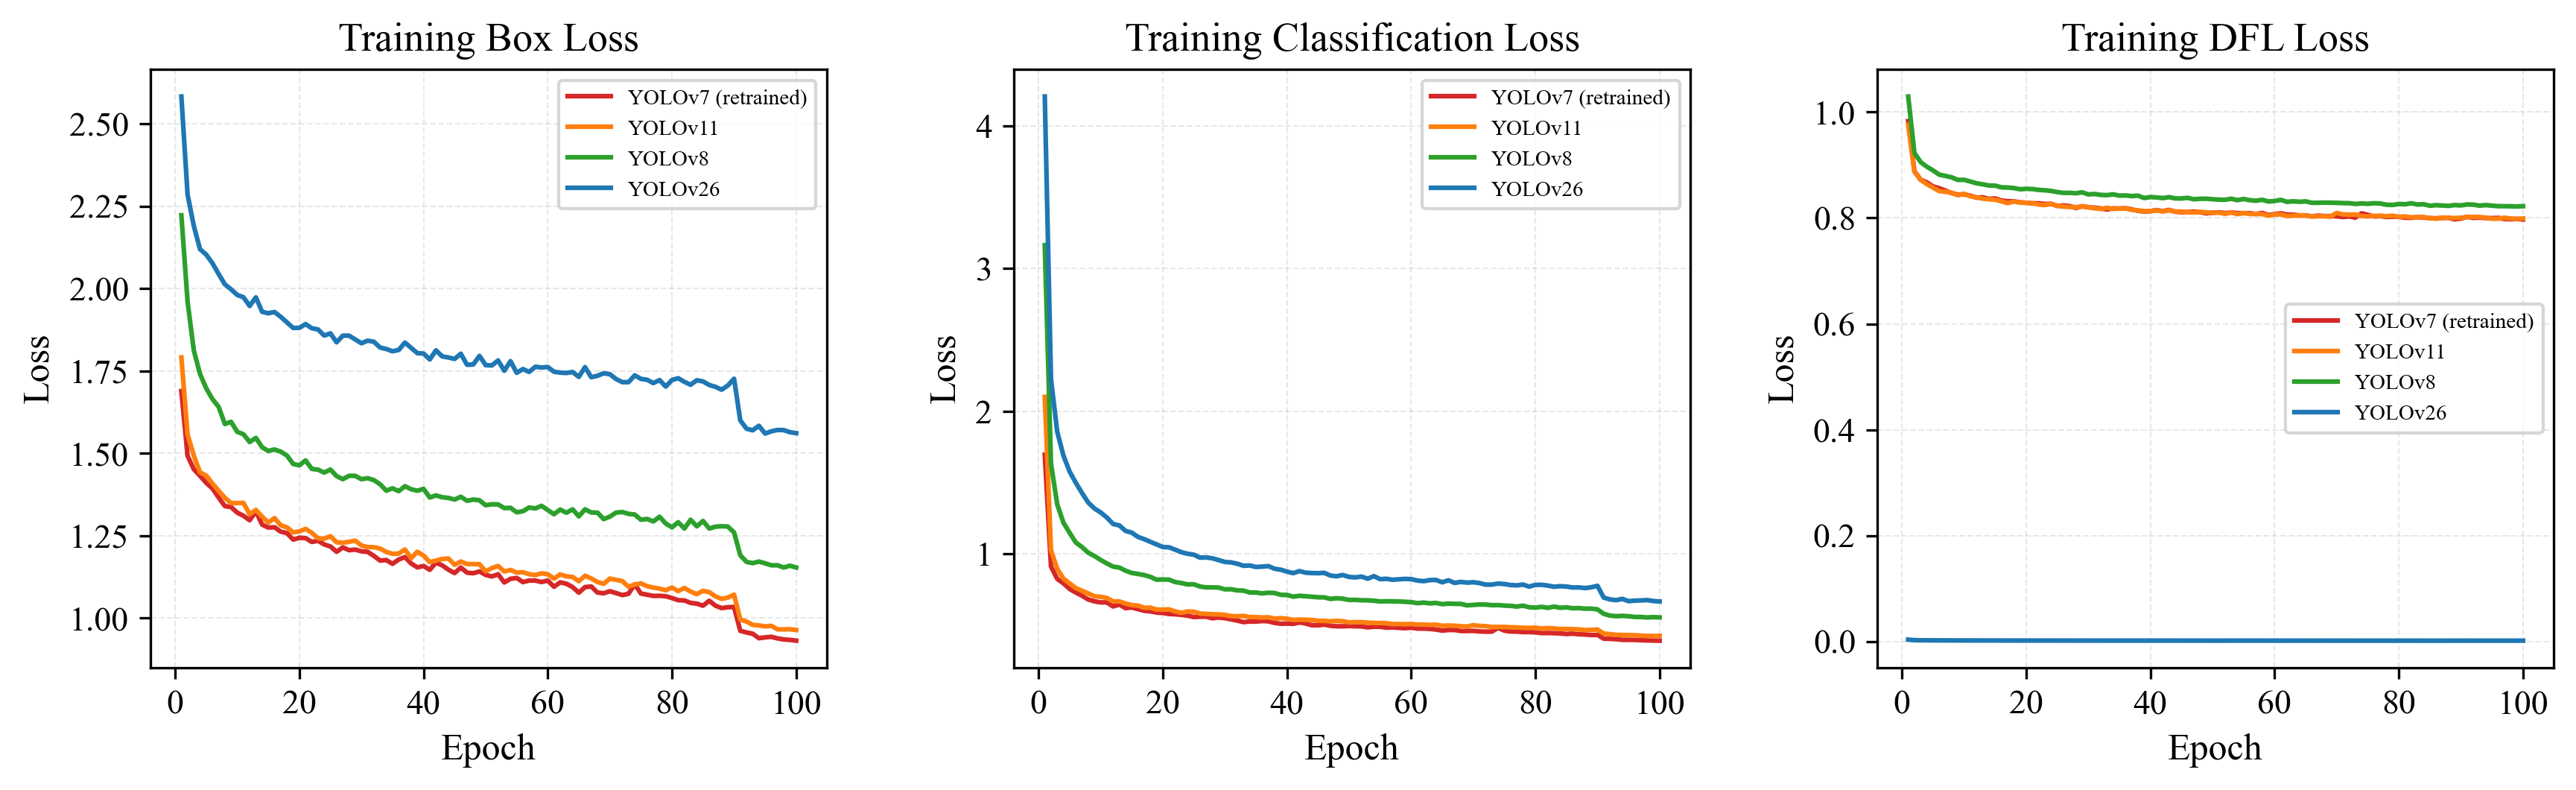
\includegraphics[width=\textwidth]{src/images/figures/yolo_15class_train_loss.png}
    \caption{Comparison of training loss (four YOLO architectures)}
    \label{fig:15class-train-loss}
\end{figure}

\begin{figure}[H]
    \centering
    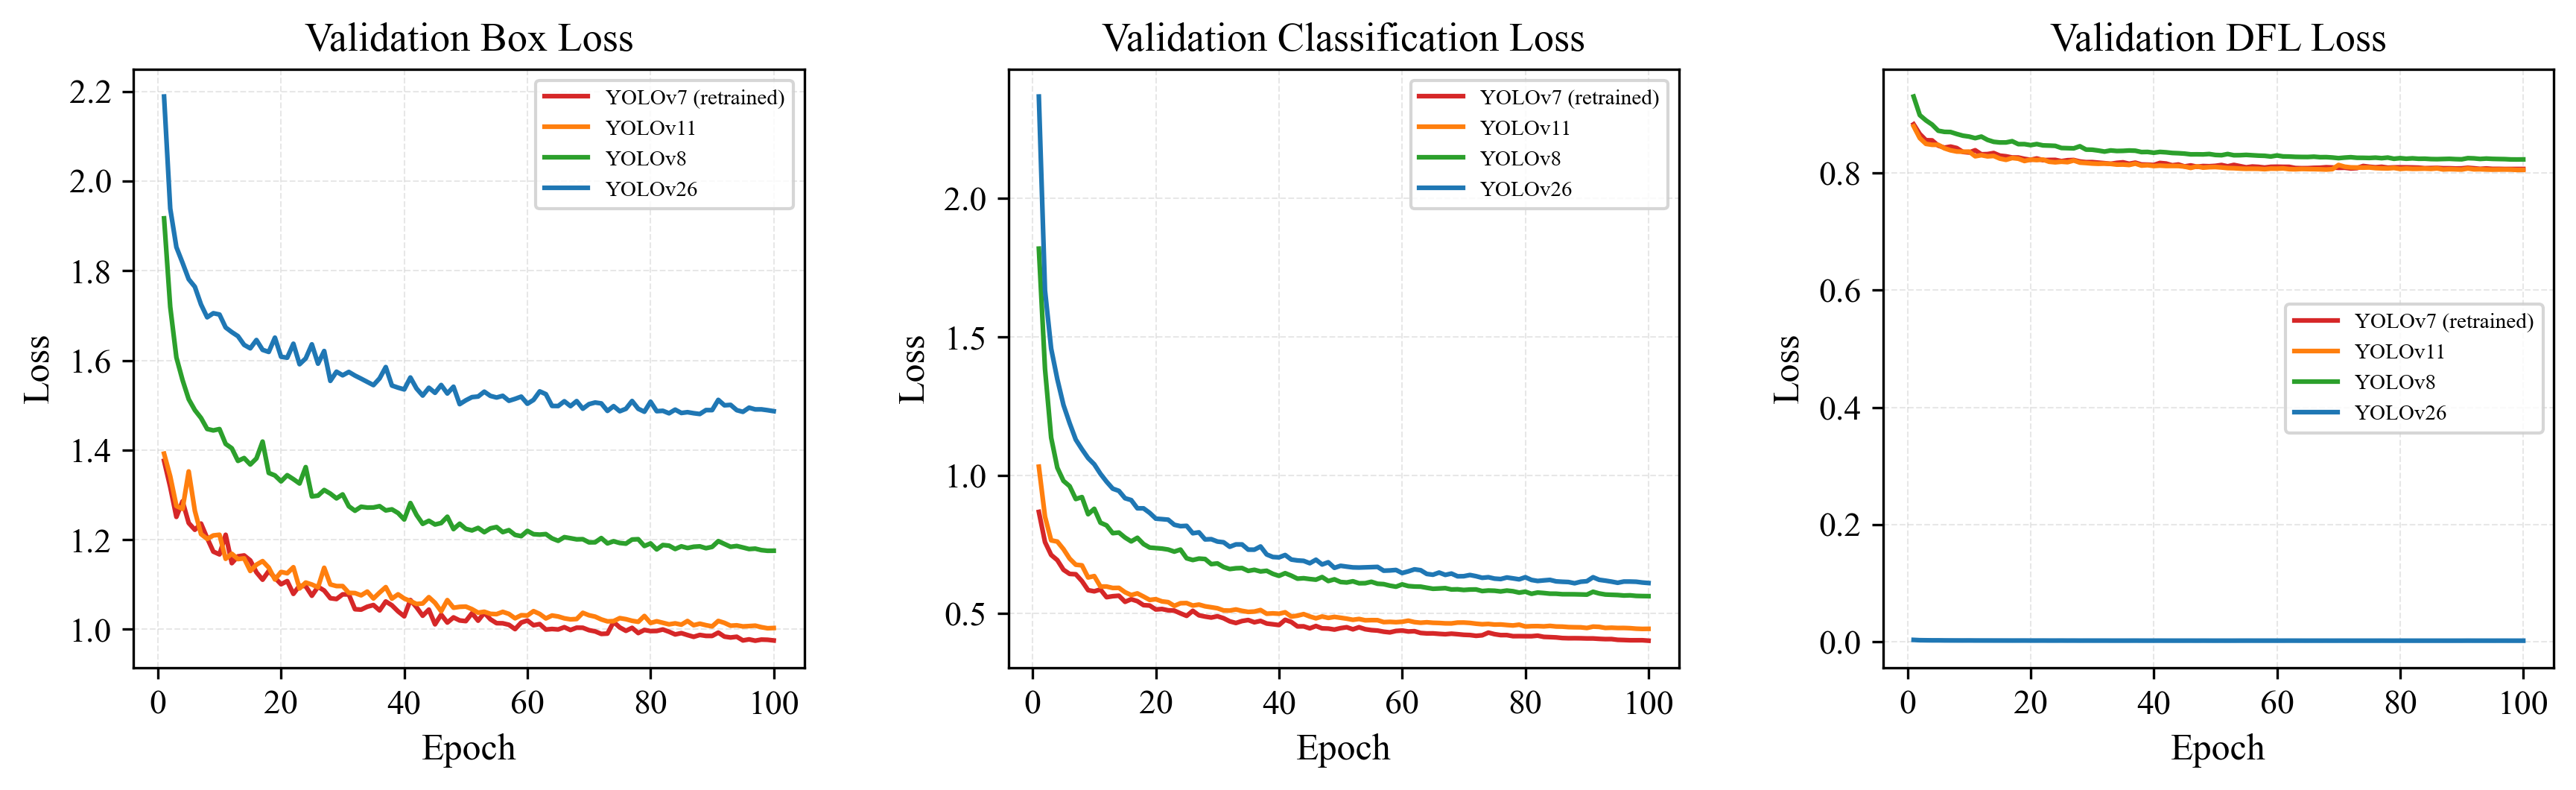
\includegraphics[width=\textwidth]{src/images/figures/yolo_15class_val_loss.png}
    \caption{Comparison of validation loss (four YOLO architectures)}
    \label{fig:15class-val-loss}
\end{figure}

\cref{fig:15class-train-loss} and \cref{fig:15class-val-loss} show the training and validation loss for all four models. The training and validation loss for YOLOv7 (retrained) and YOLOv11 declined sharply and reached the lowest value among the four architectures.

\subsection{Performance Metrics: 15-Class Models}

\begin{figure}[H]
    \centering
    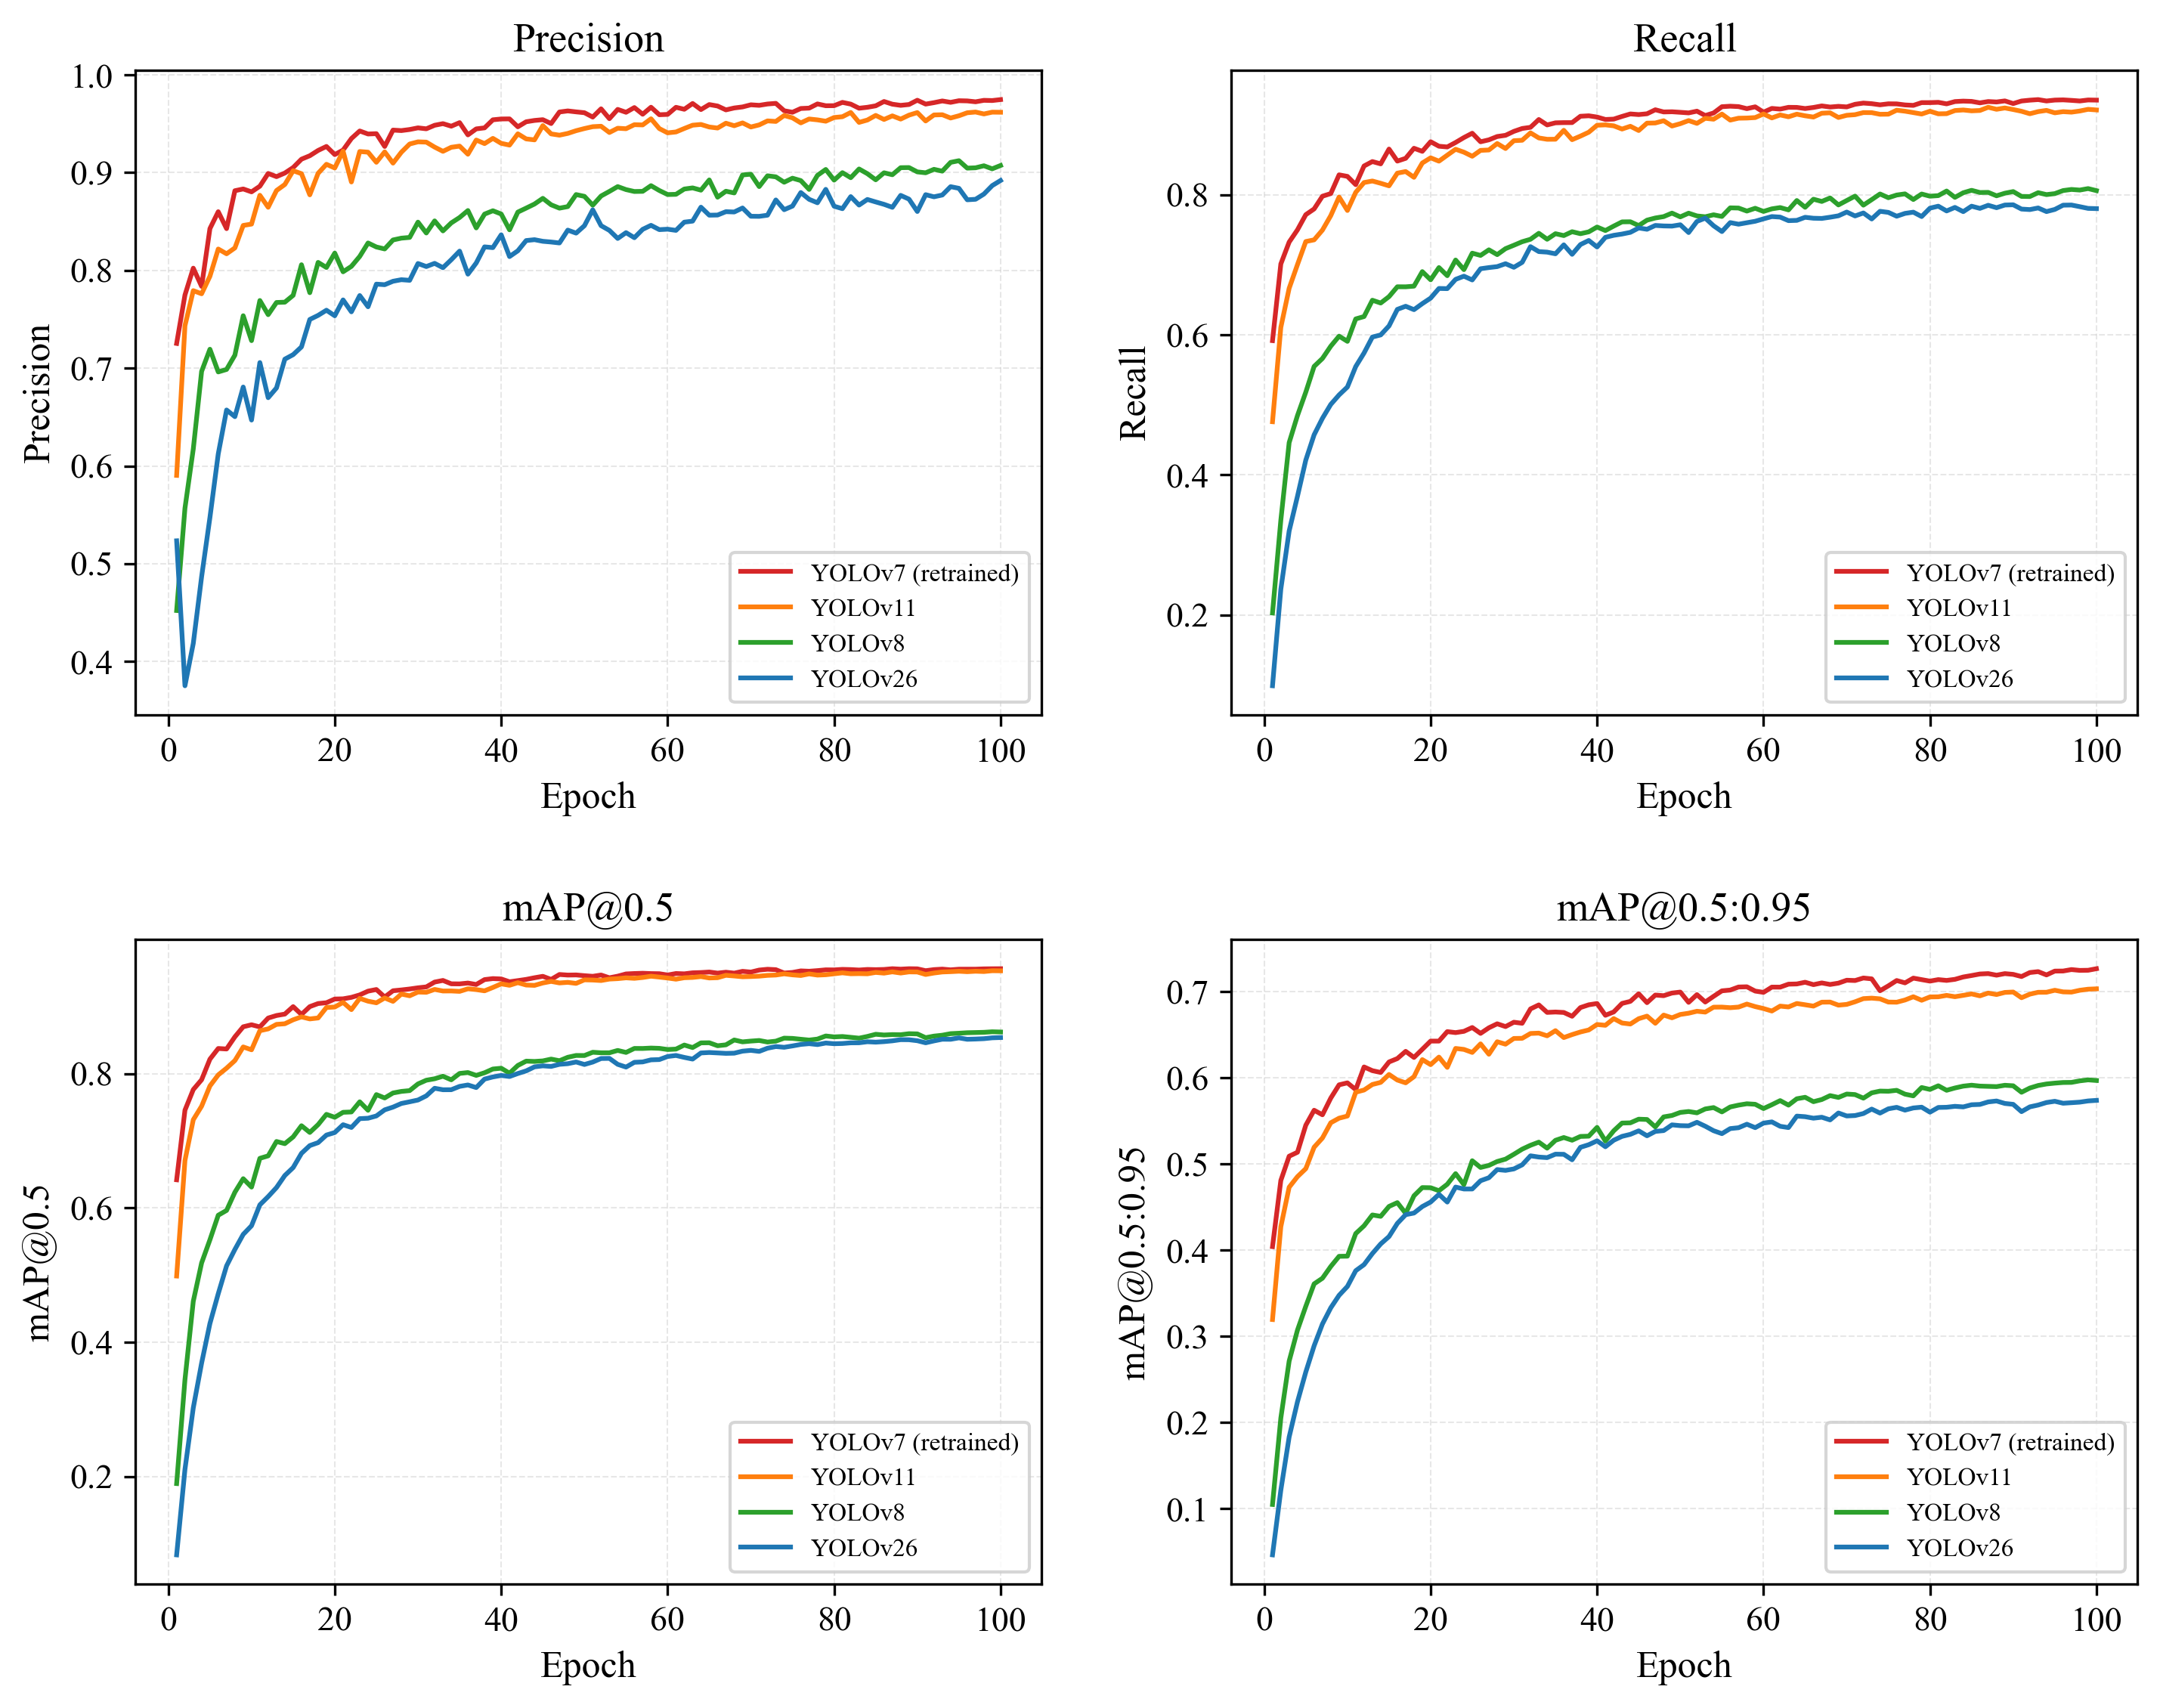
\includegraphics[width=\textwidth]{src/images/figures/yolo_15class_training_curves.png}
    \caption{Performance metrics vs epochs on the consolidated dataset}
    \label{fig:15class-training-curves}
\end{figure}

\cref{fig:15class-training-curves} plots precision, recall, mAP@0.5, and mAP@0.5:0.95 for 100 epochs for all four YOLO architectures. YOLOv7 (retrained) and YOLOv11 plateau at around epoch 40 to 50 reaching their near-maximum values  for each performance metric, all of which are consistently higher than the other two YOLO architectures. 

\subsection{Quantitative Results Comparison for 15-Class Dataset}

\begin{table}[H]
    \centering
    \caption{Final epoch performance comparison of four \gls{yolo} architectures on the consolidated dataset}
    \label{table:yolo-15class-comparison}
    \begin{tabular}{lrrrr}
        \toprule
        \textbf{Metric} & \textbf{YOLOv7 (retrained)} & \textbf{YOLOv11} & \textbf{YOLOv8} & \textbf{YOLOv26} \\
        \midrule
        Precision        & \textbf{0.9747} & 0.9617 & 0.9073 & 0.8919 \\
        Recall           & \textbf{0.9350} & 0.9209 & 0.8058 & 0.7801 \\
        \gls{map}@0.5    & \textbf{0.9562} & 0.9531 & 0.8620 & 0.8537 \\
        \gls{map}@0.5:0.95 & \textbf{0.7266} & 0.7033 & 0.5969 & 0.5738 \\
        Epochs           & 100 & 100 & 100 & 100 \\
        \bottomrule
    \end{tabular}
\end{table}

\begin{figure}[H]
    \centering
    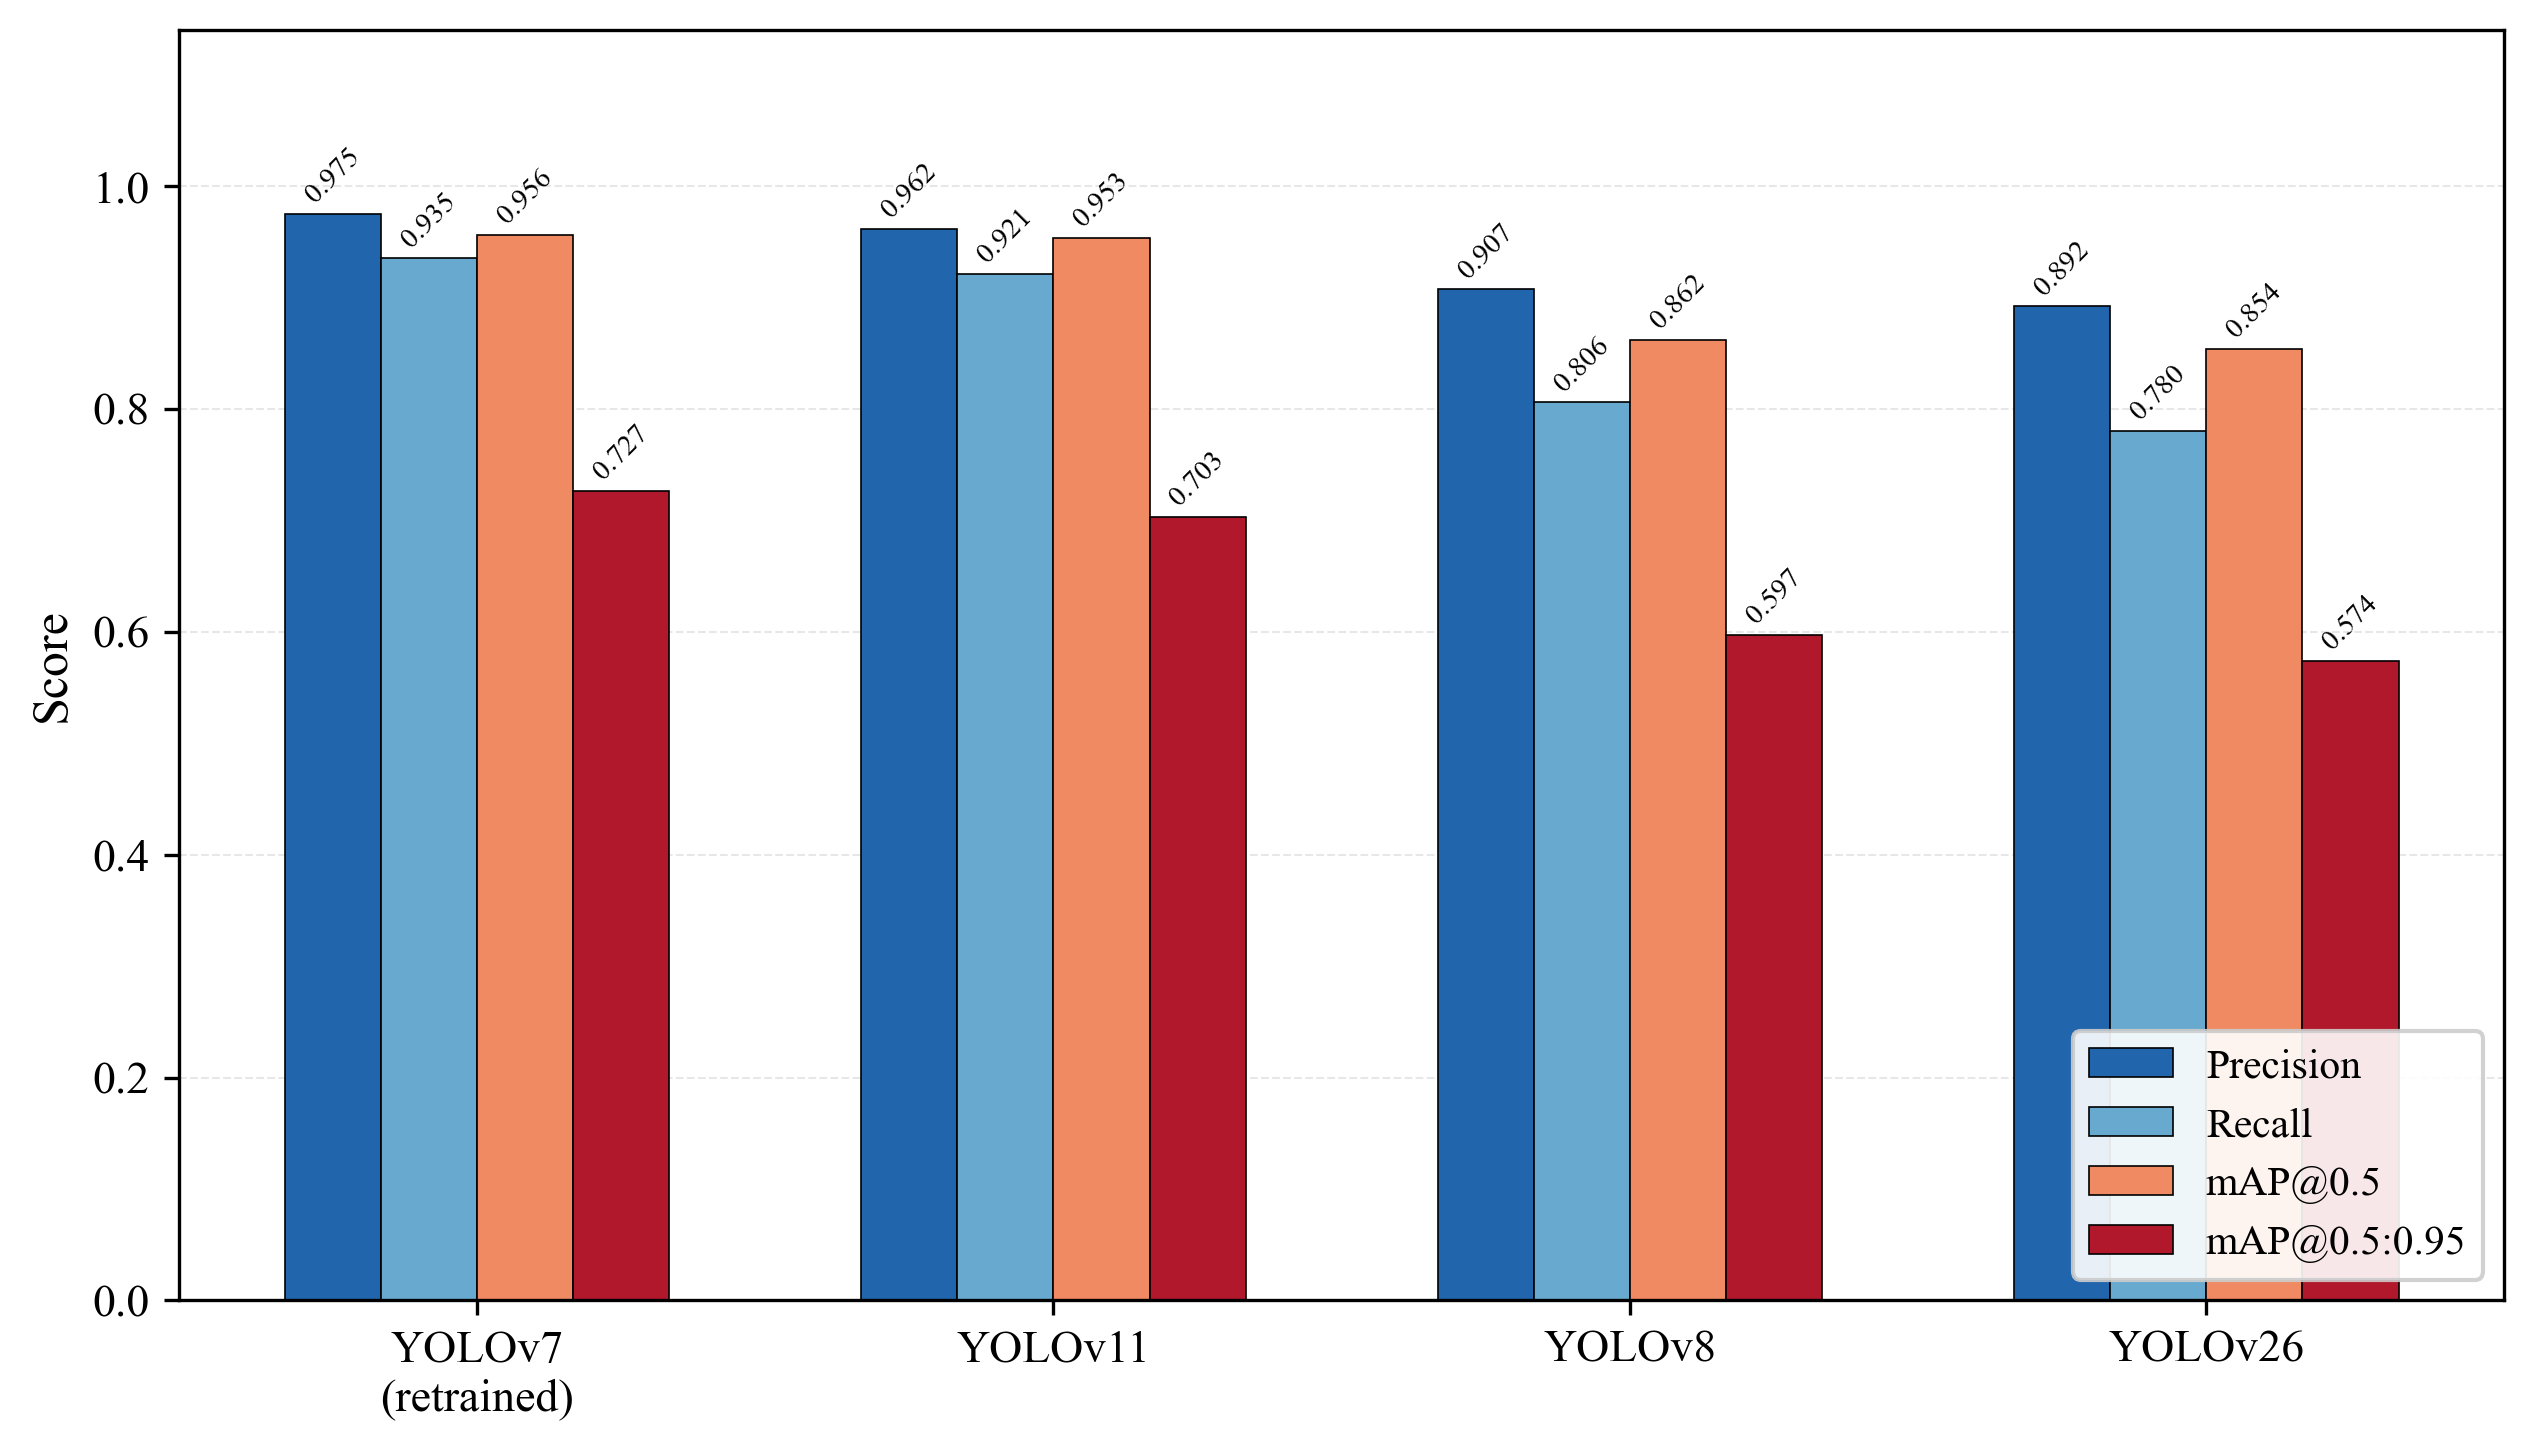
\includegraphics[width=\textwidth]{src/images/figures/yolo_15class_final_bar.png}
    \caption{Final-epoch performance metrics for four \gls{yolo} architectures on the 15-class dataset}
    \label{fig:15class-final-bar}
\end{figure}

\cref{table:yolo-15class-comparison} displays the values of performance metrics at the final epoch for all four YOLO architectures. \cref{fig:15class-final-bar} displays the same data in a bar chart. YOLOv7 (retrained) is clearly the best models based on all the mentioned metrics, with YOLOv11 following closely. The target value of mAP@0.5 (0.95) is achieved by both of them.

\subsection{Impact of Class Taxonomy Consolidation}

\begin{table}[H]
    \centering
    \caption{Effect of class consolidation on YOLOv7 performance}
    \label{table:class-impact}
    \begin{tabular}{lrrr}
        \toprule
        \textbf{Metric} & \textbf{61-Class} & \textbf{15-Class} & \textbf{Improvement} \\
        \midrule
        Precision        & 0.93 & 0.9747 & +4.8\% \\
        Recall           & 0.78 & 0.9350 & +19.9\% \\
        \gls{map}@0.5    & 0.83 & 0.9562 & +15.2\% \\
        \gls{map}@0.5:0.95 & 0.60 & 0.7266 & +21.1\% \\
        \bottomrule
    \end{tabular}
\end{table}

\begin{figure}[H]
    \centering
    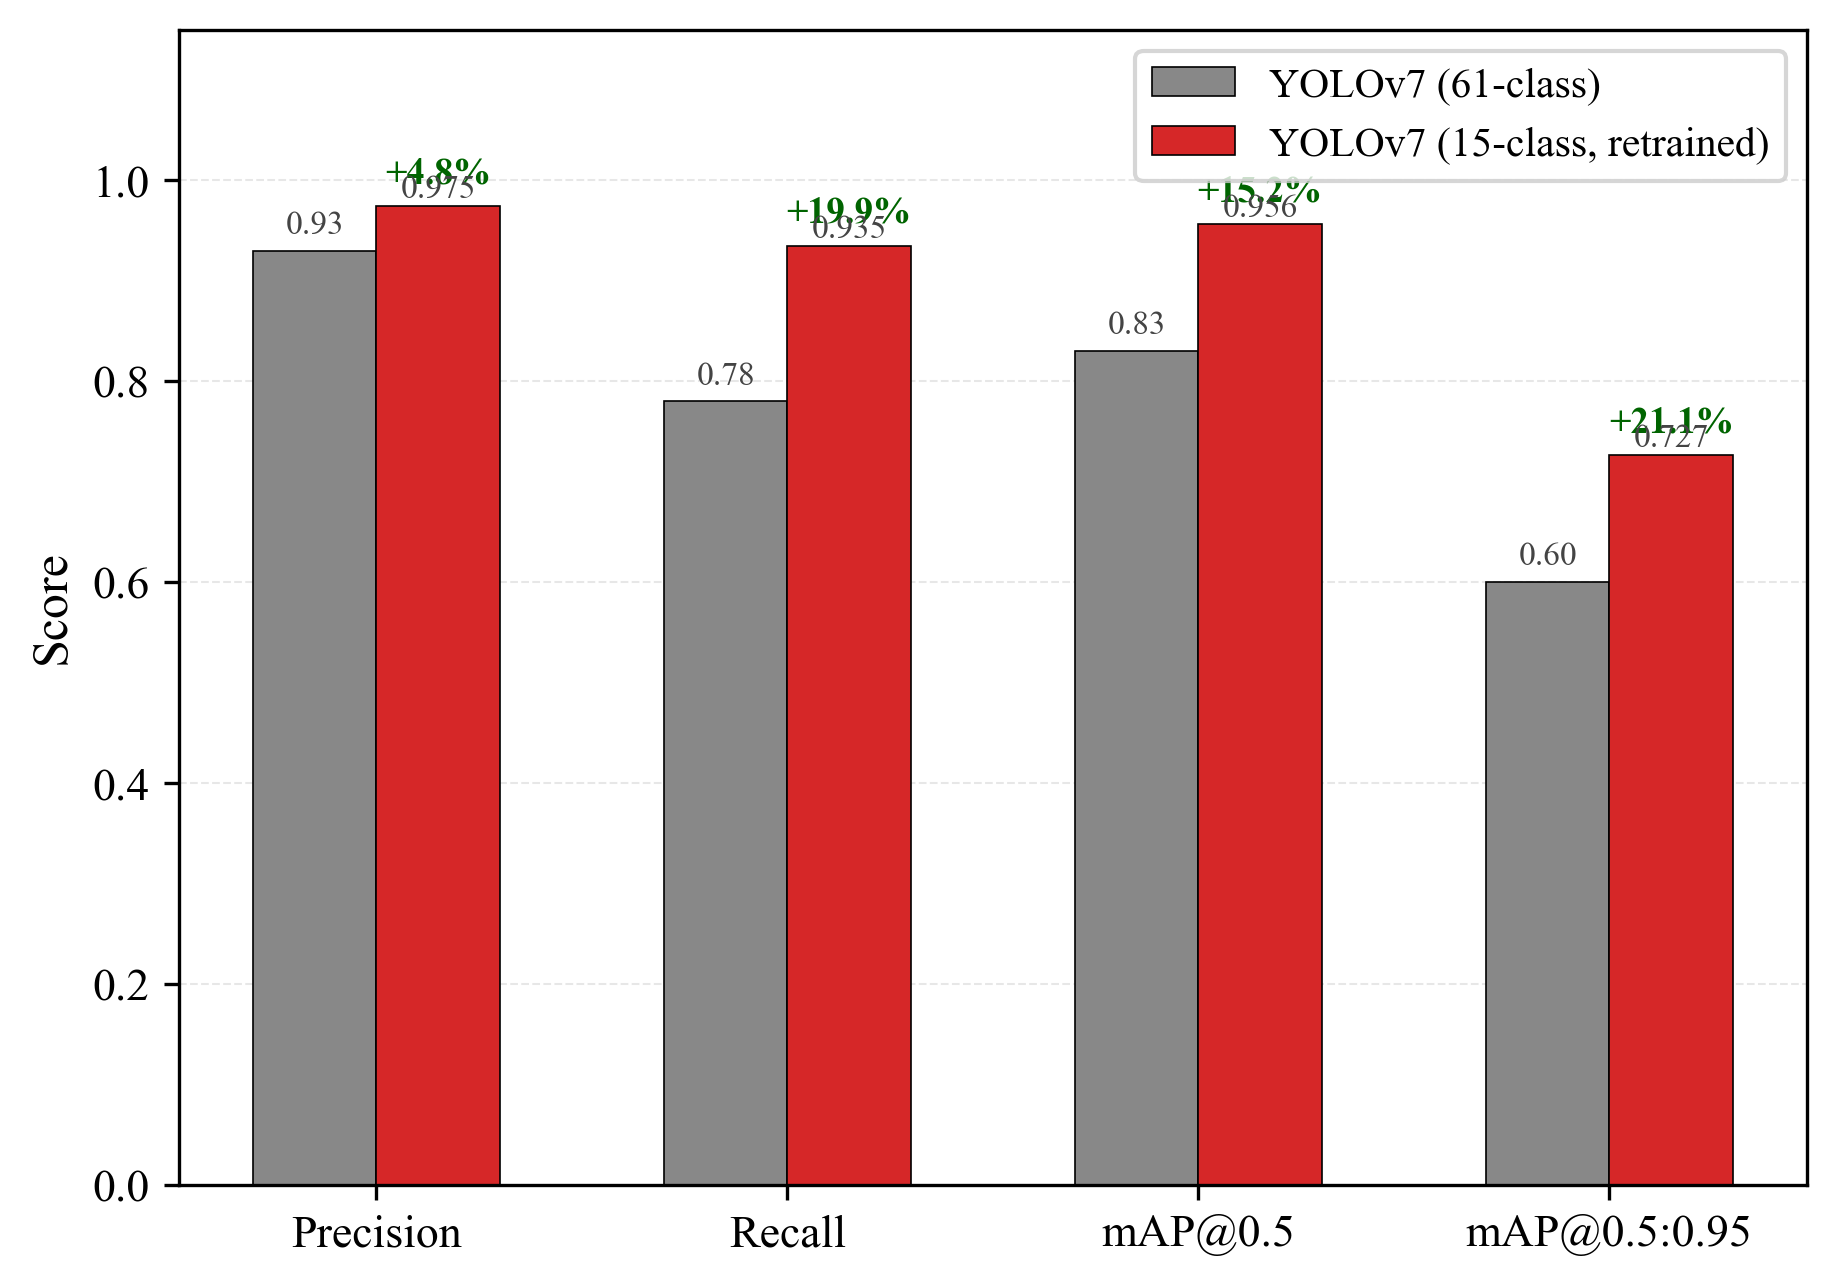
\includegraphics[width=0.85\textwidth]{src/images/figures/yolo_class_impact.png}
    \caption{Effect of class consolidation on YOLOv7 performance}
    \label{fig:class-impact}
\end{figure}

\cref{fig:class-impact} and \cref{table:class-impact} show the improvement in performance metrics for YOLOv7 due to consolidation of classes from 61 to 15. This shows that the consolidation, although decreased the nuances in different components, ultimately improved the detection performance.

\section{Holistic Object Detection Comparison}

\begin{table}[H]
    \centering
    \caption{Comparison of performance of all object detection models}
    \label{table:yolo-full-comparison}
    \begin{tabular}{llrrrr}
        \toprule
        \textbf{Model} & \textbf{Classes} & \textbf{Precision} & \textbf{Recall} & \textbf{\gls{map}@0.5} & \textbf{\gls{map}@0.5:0.95} \\
        \midrule
        YOLOv5 & 61 & 0.84 & 0.62 & 0.61 & 0.41 \\
        YOLOv7 & 61 & 0.93 & 0.78 & 0.83 & 0.60 \\
        YOLOv8 & 15 & 0.9073 & 0.8058 & 0.8620 & 0.5969 \\
        YOLOv26 & 15 & 0.8919 & 0.7801 & 0.8537 & 0.5738 \\
        YOLOv11 & 15 & 0.9617 & 0.9209 & 0.9531 & 0.7033 \\
        \textbf{YOLOv7 (retrained)} & \textbf{15} & \textbf{0.9747} & \textbf{0.9350} & \textbf{0.9562} & \textbf{0.7266} \\
        \bottomrule
    \end{tabular}
\end{table}

\begin{figure}[H]
    \centering
    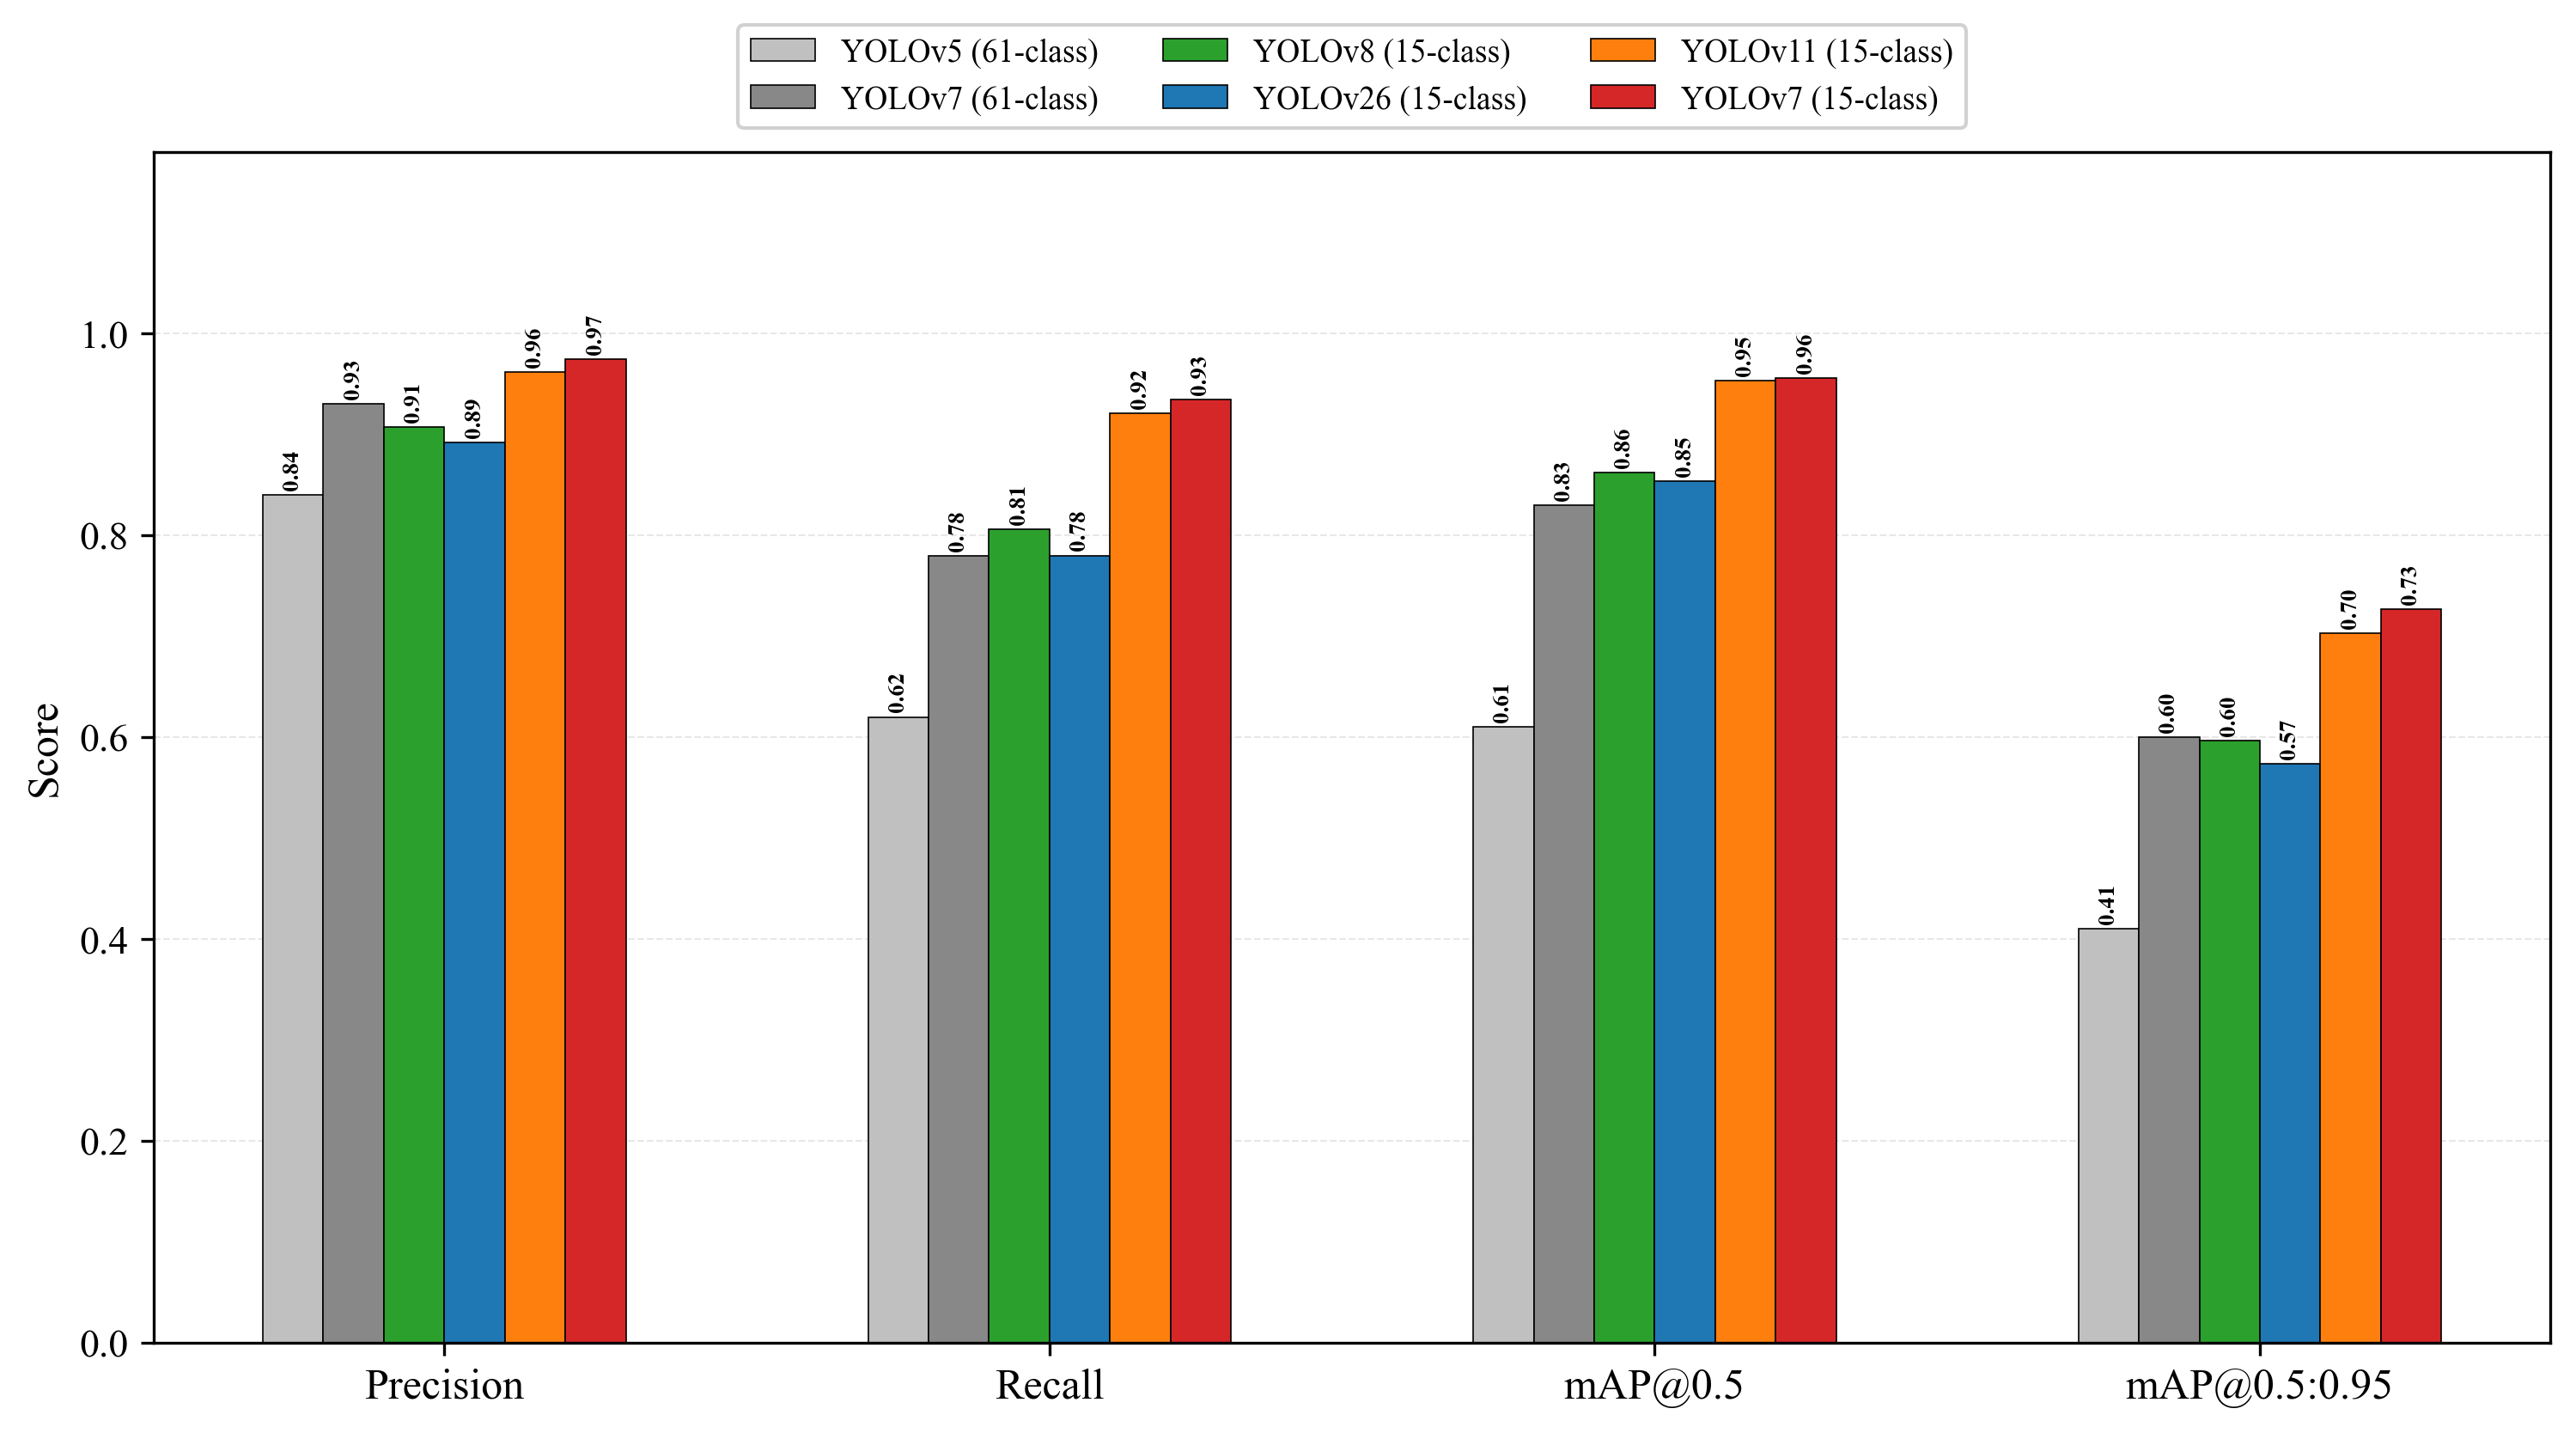
\includegraphics[width=\textwidth]{src/images/figures/yolo_full_comparison_bar.png}
    \caption{Comparison of performance of all object detection models}
    \label{fig:yolo-full-bar}
\end{figure}

\cref{table:yolo-full-comparison} and \cref{fig:yolo-full-bar} respectively tabulate and display the results based on all selected performance metrics for all architectures and class taxonomies.

\subsection{Radar Visualization of Top Models}

\begin{figure}[H]
    \centering
    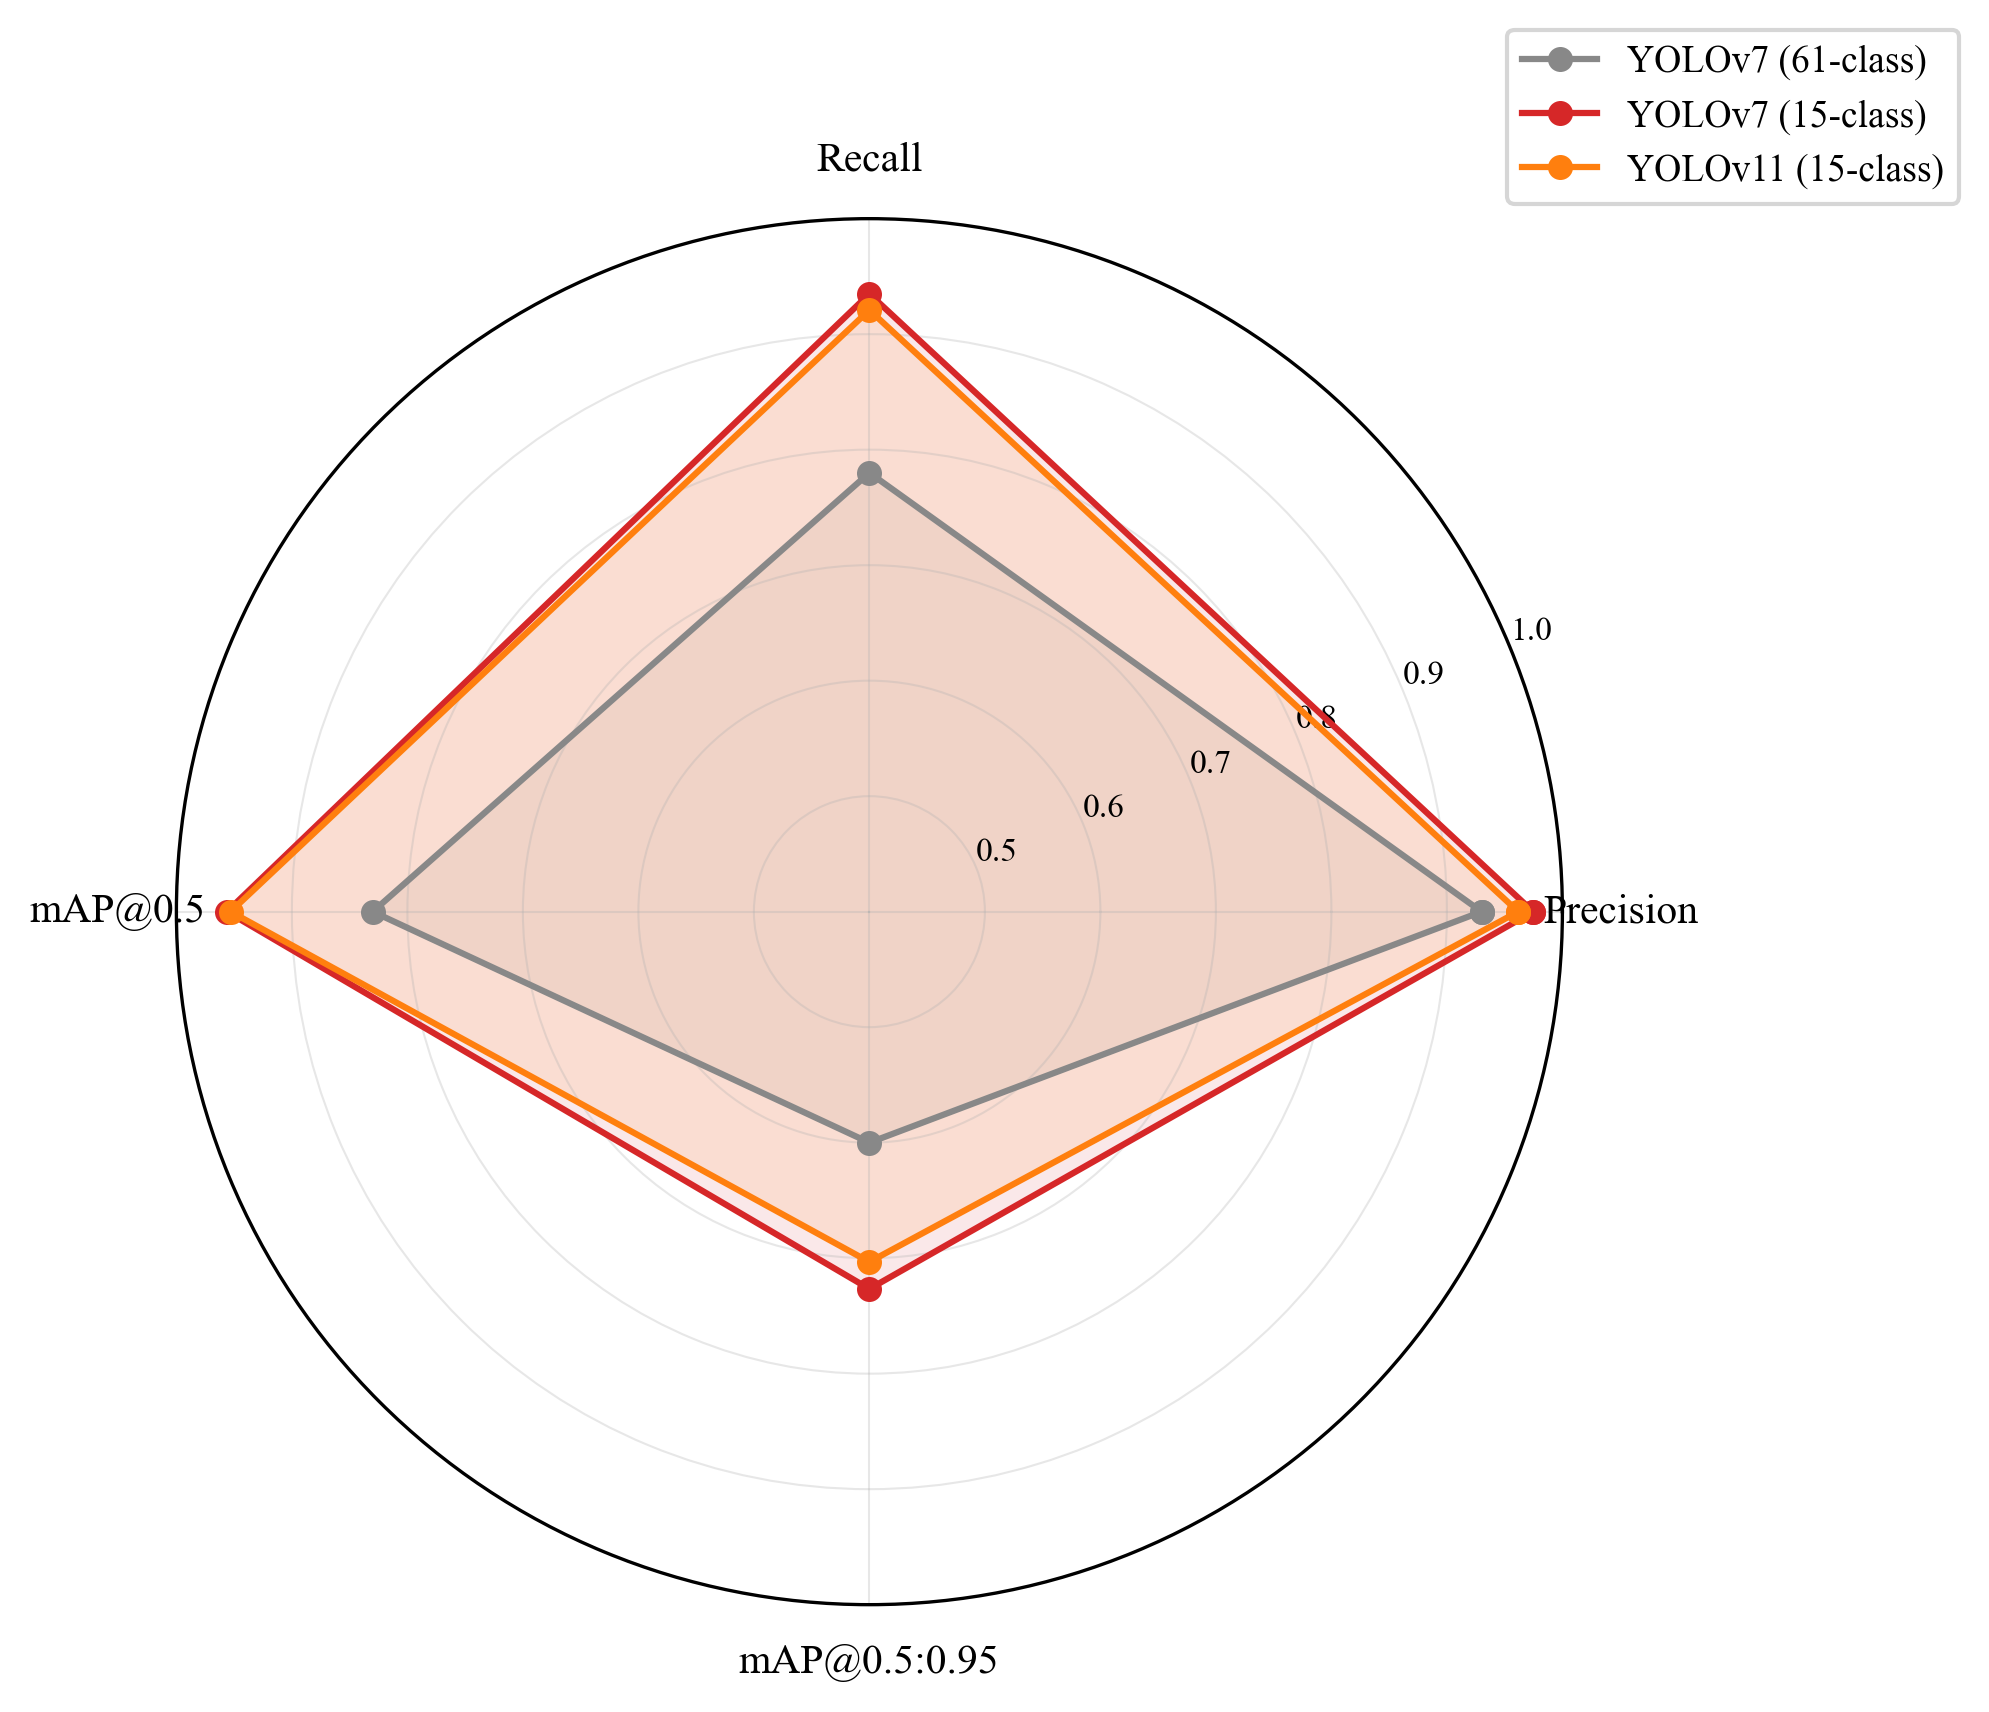
\includegraphics[width=0.65\textwidth]{src/images/figures/yolo_radar_comparison.png}
    \caption{Radar chart comparing the three best detection configurations across four performance metrics}
    \label{fig:yolo-radar}
\end{figure}

\cref{fig:yolo-radar} renders a radar chart of the three strongest configurations. YOLOv7 (61-class) lags visibly in recall (0.78 versus 0.93+), whereas both 15-class models fill out nearly the entire performance envelope. The retrained YOLOv7 (15-class) marginally outperforms YOLOv11 across all axes, making it the model of choice for the final pipeline.

Overall, from all these findings, it is evident that YOLOv7 (retrained on the 15-class taxonomy) is the optimal object detection model for this project. This also goes to show that class taxonomy might matter more than the architecture at times.

\subsection{Confusion Matrix for the retrained YOLOv7}

\begin{figure}[H]
    \centering
    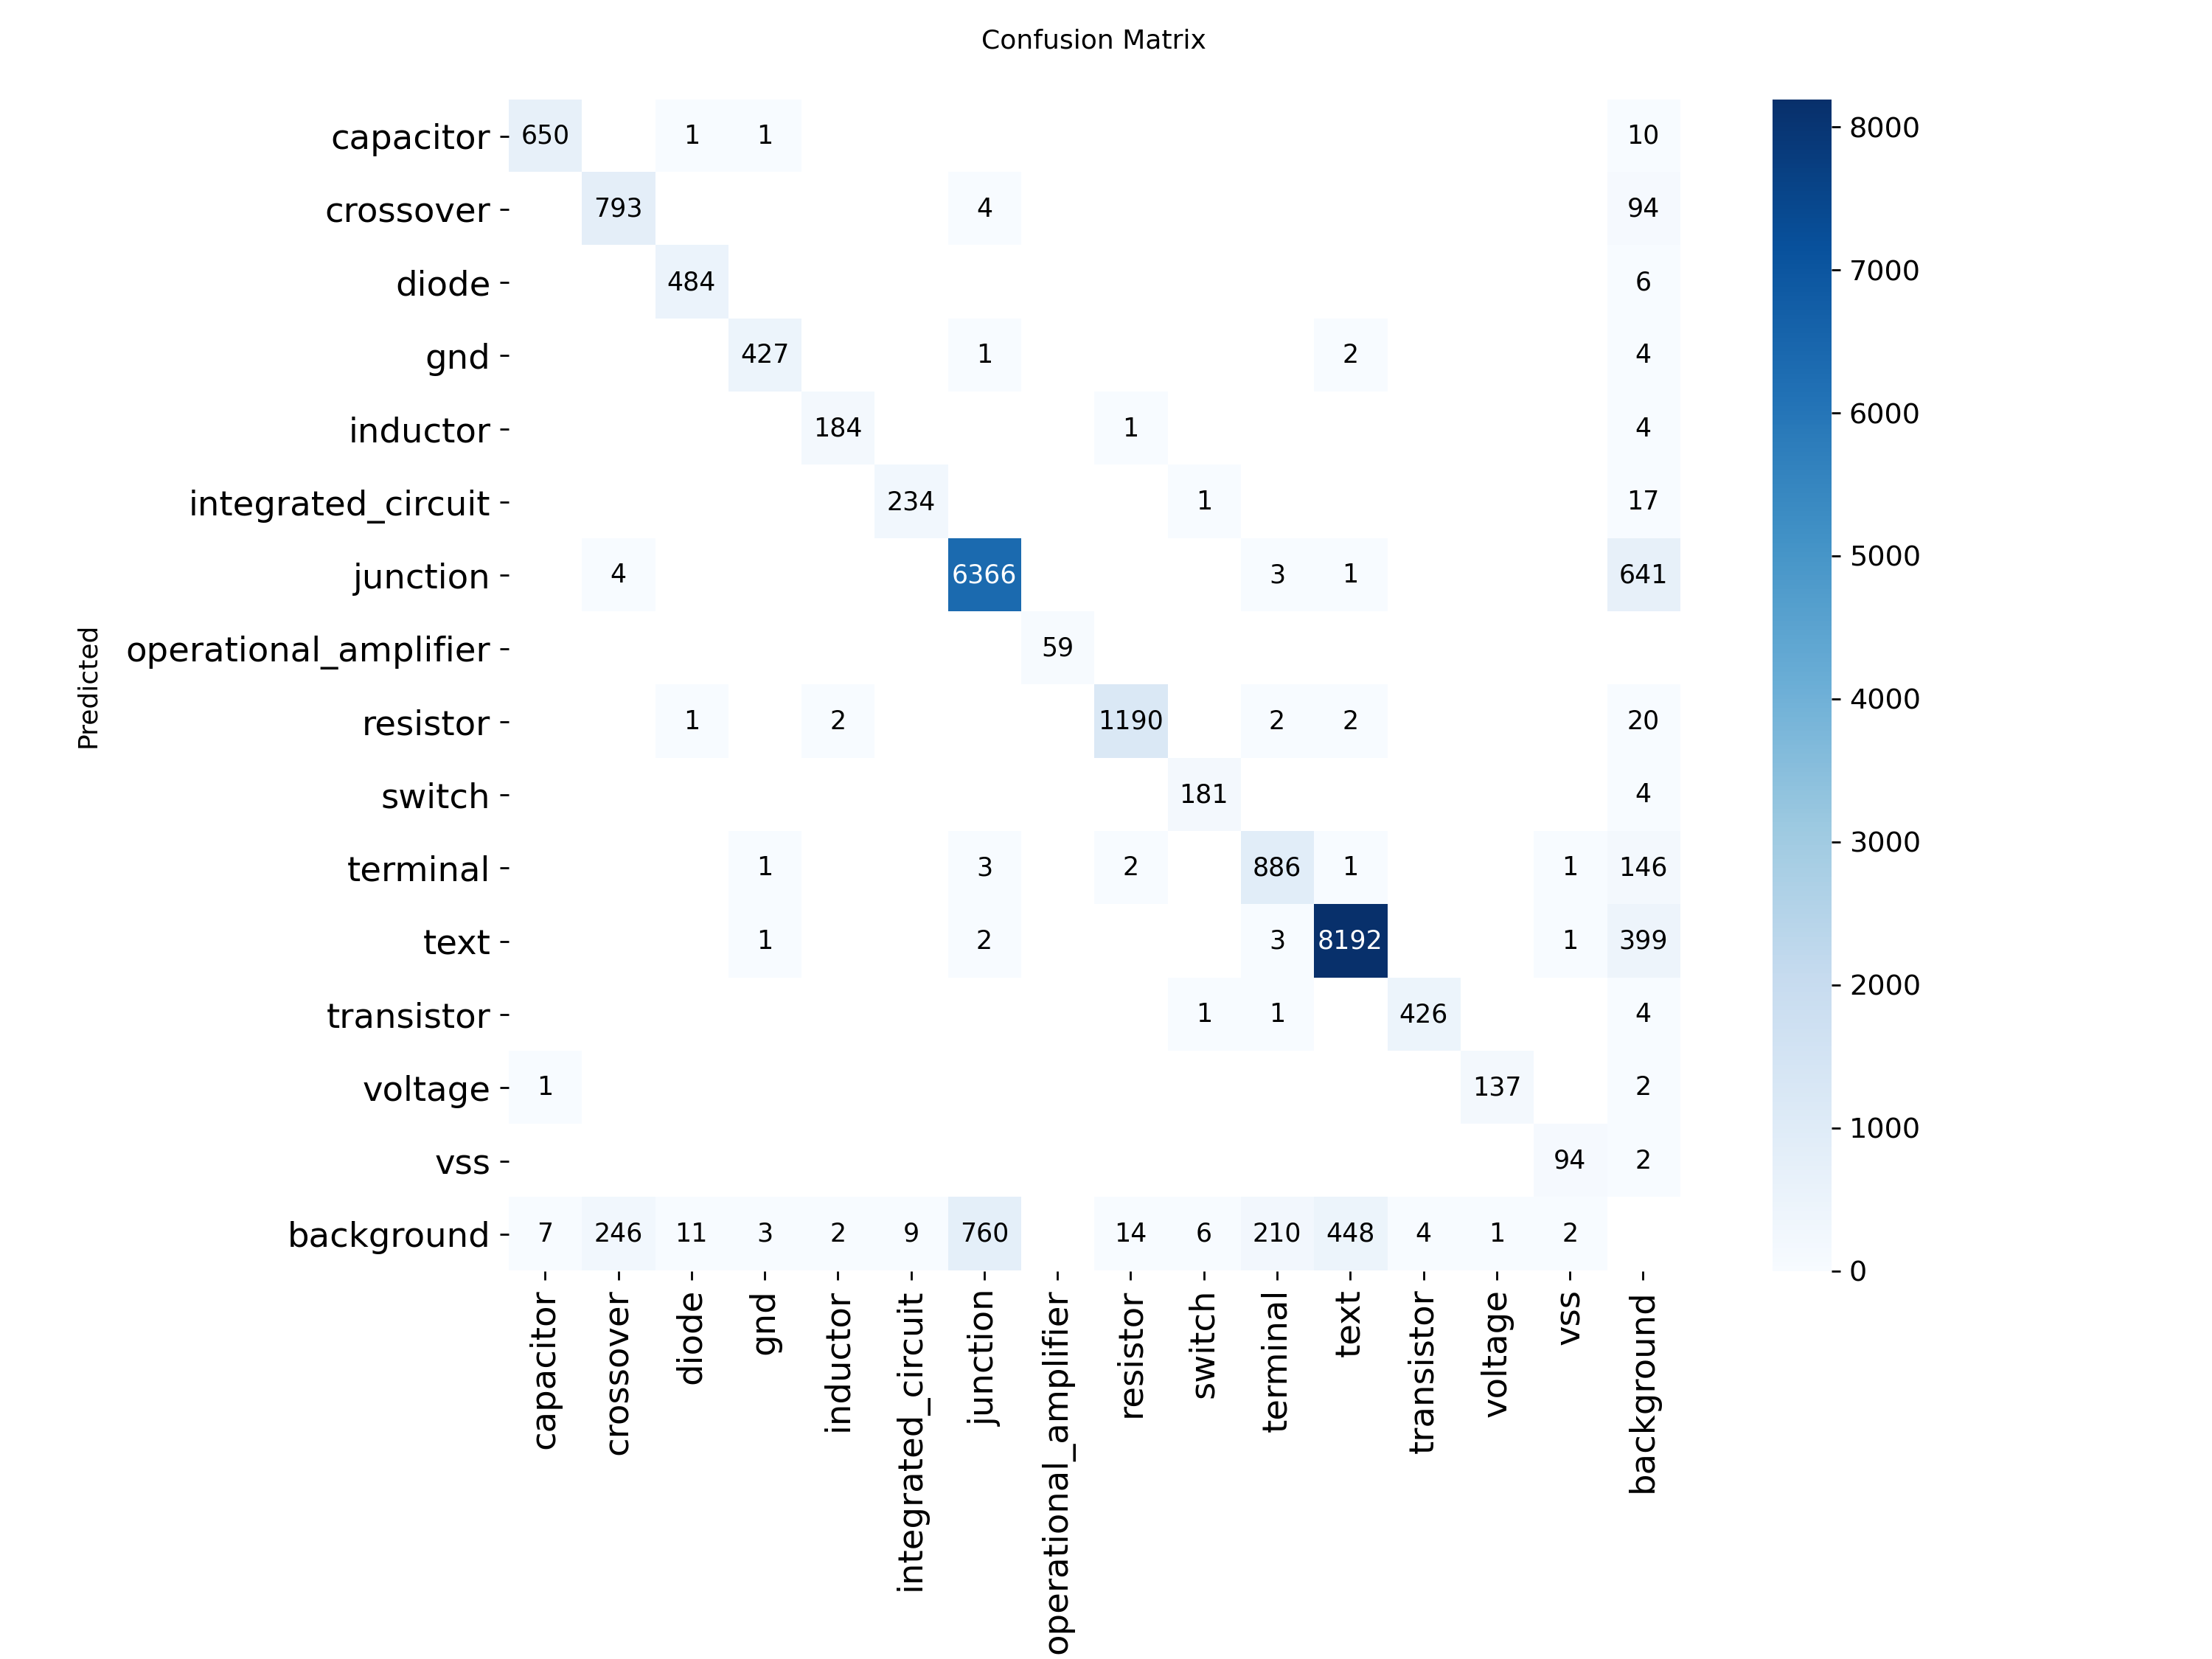
\includegraphics[width=\textwidth]{src/images/figures/confusion_matrix_retrained_yolov7.png}
    \caption{Confusion Matrix for the retrained YOLOv7}
    \label{fig:confusion-matrix-retrained-yolov7}
\end{figure}

\cref{fig:confusion-matrix-retrained-yolov7} demonstrates the confusion matrix for the retrained YOLOv7 (15 classes). It has a darker main diagonal and very light off-diagonals, which means that the model exhibits strong class separability with minimal inter-class confusion.

\section{Retrained YOLOv7 Demonstration}
\begin{figure}[H]
    \centering
    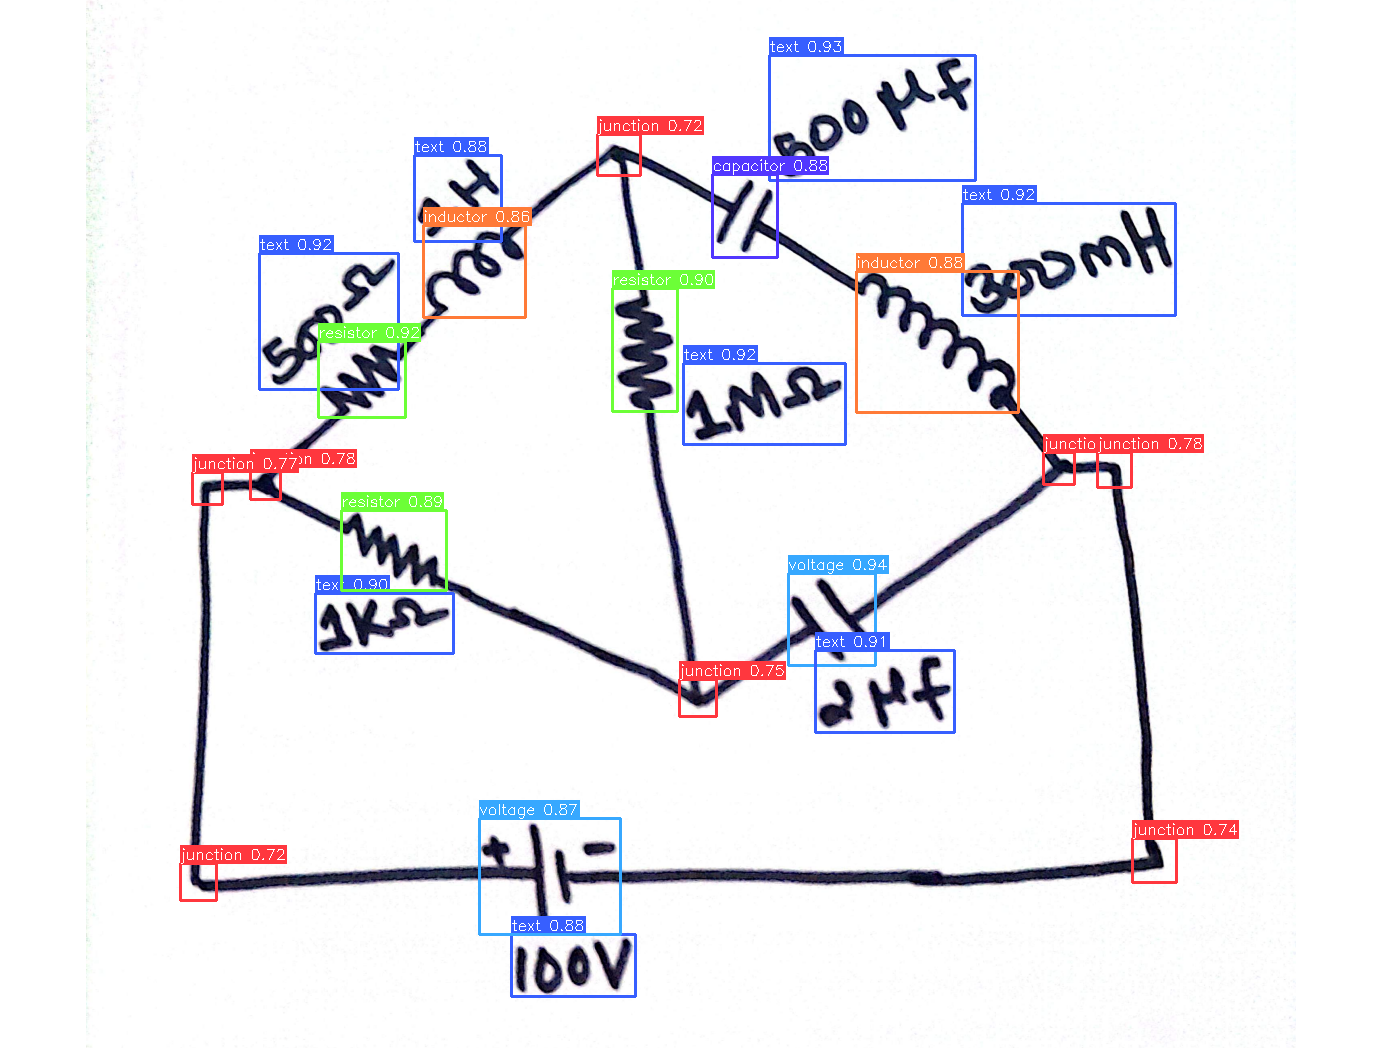
\includegraphics[width=\textwidth]{src/images/figures/retrained_yolov7_result1.png}
    \caption{Retrained YOLOv7 Result (i)}
    \label{fig:retrained-yolov7-result-1}
\end{figure}

\begin{figure}[H]
    \centering
    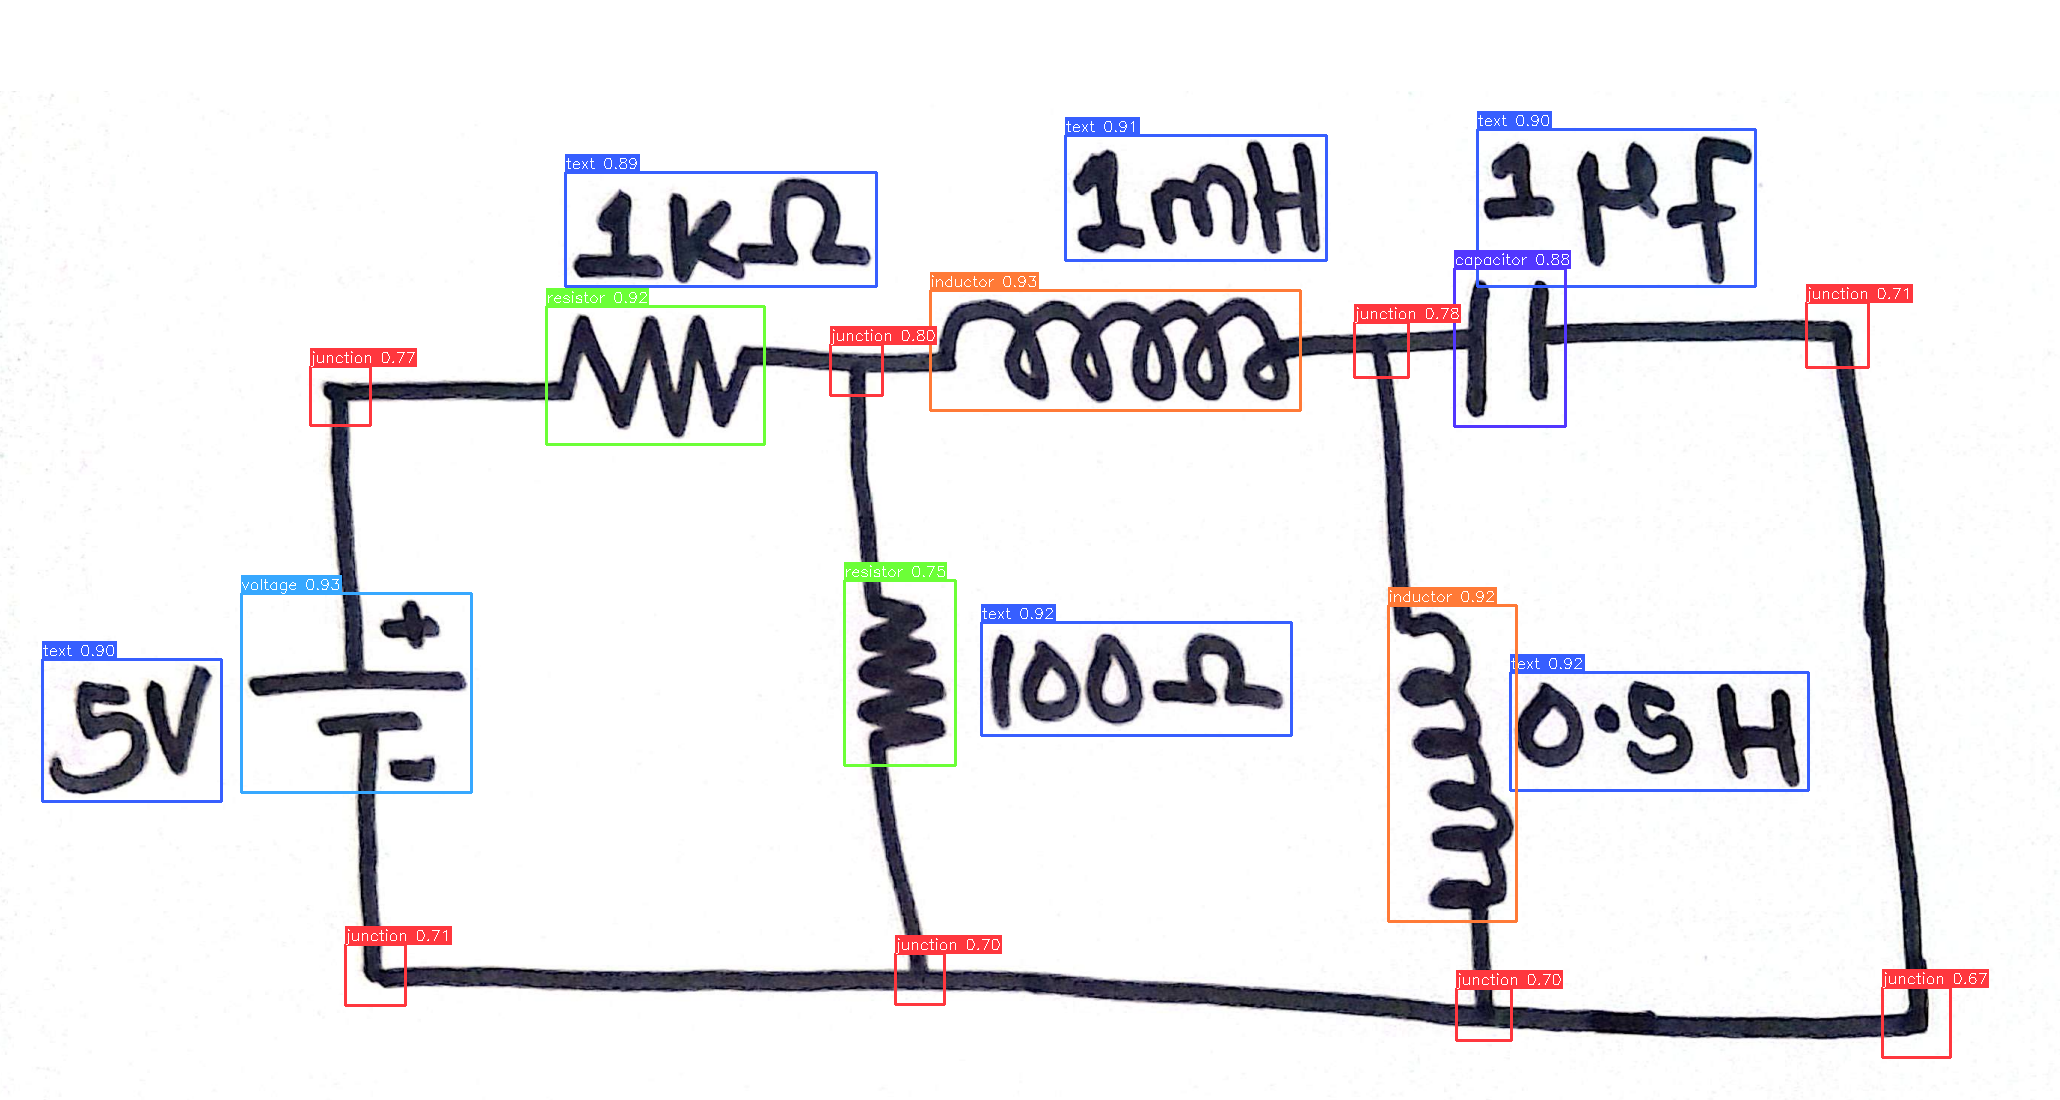
\includegraphics[width=\textwidth]{src/images/figures/retrained_yolov7_result2.png}
    \caption{Retrained YOLOv7 Result (ii)}
    \label{fig:retrained-yolov7-result-2}
\end{figure}

\cref{fig:retrained-yolov7-result-1} and \cref{fig:retrained-yolov7-result-2} show the results of the retrained YOLOv7 on two random test images. The model successfully detects and classifies all components in both images with high confidence scores. These results visually confirm the quantitative metrics and demonstrate the model's effectiveness in real-world scenarios.

\section{Custom OCR Results and Analysis}
\subsection{Custom OCR Training Loss Curve}

\begin{figure}[H]
    \centering
    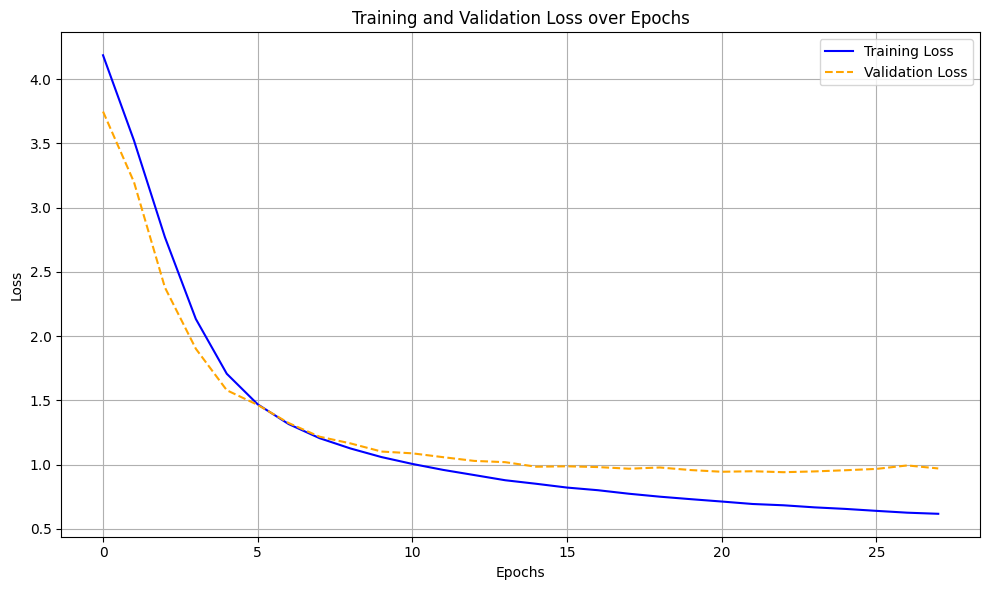
\includegraphics[width=\textwidth]{src/images/figures/custom_OCR_loss_curve.png}
    \caption{Training Loss vs Epochs (Custom \gls{ocr})}
    \label{fig:custom-ocr-loss-curve}
\end{figure}

\cref{fig:custom-ocr-loss-curve} shows that the training loss decreases consistently throughout the 27 epochs, indicating the model is effectively memorizing the training data. There seems to be the slightest uptick in the validation loss, though, at 26 epoch indicating a hint of potential overfitting. The training was stopped at 27 epochs due to early stopping criteria being met.


\subsection{Custom OCR Performance Analysis}

\begin{figure}[H]
    \centering
    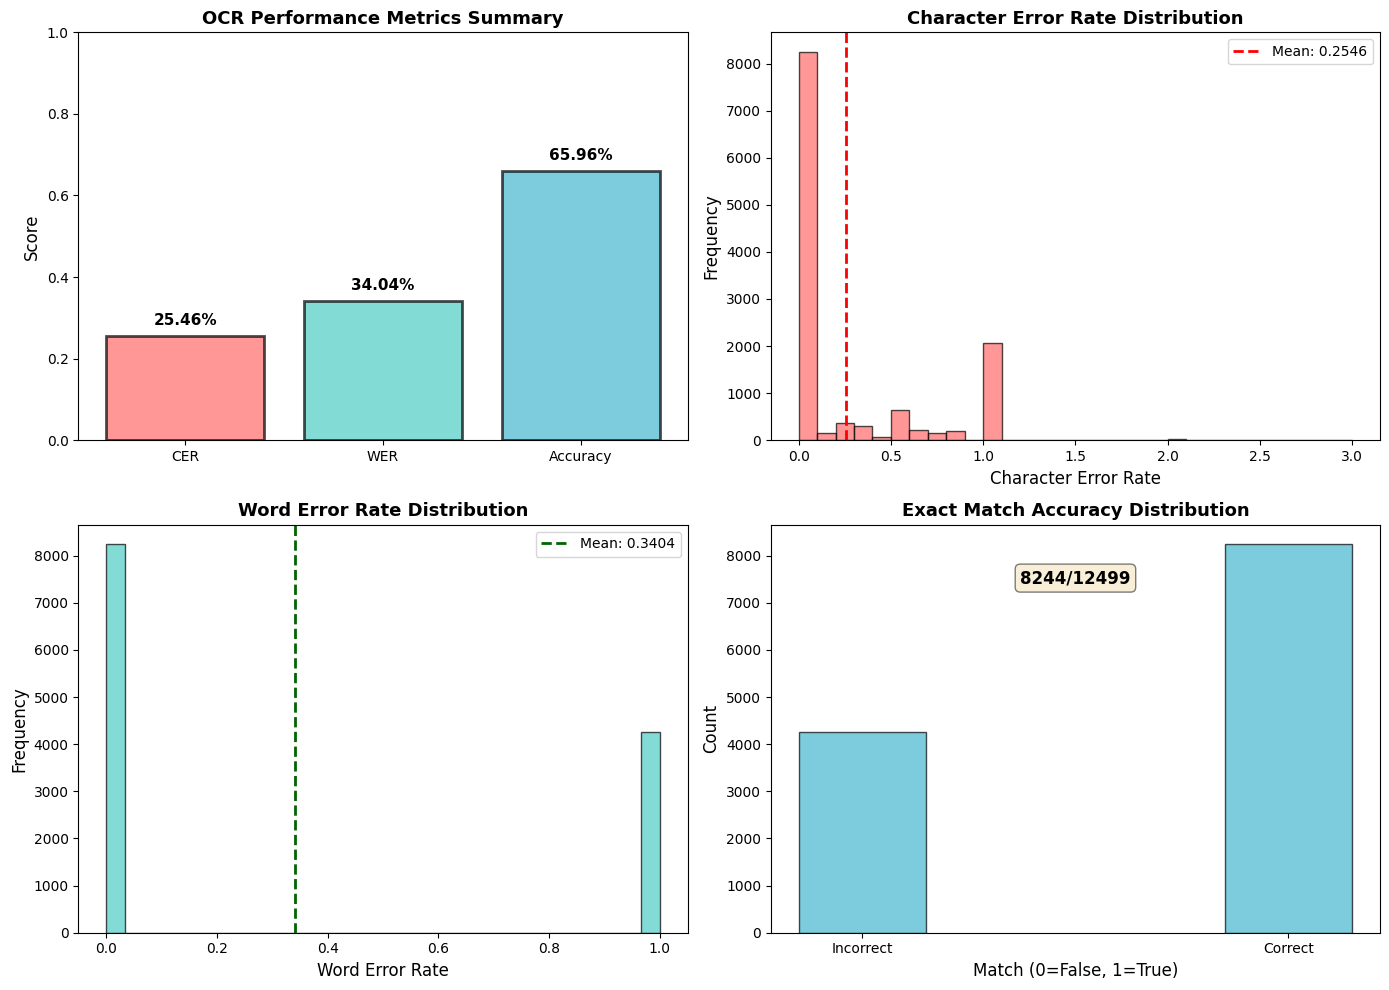
\includegraphics[width=\textwidth]{src/images/figures/cer_wer.png}
    \caption{Custom OCR Performance Metrics and their Distributions}
    \label{fig:ocr-performance-metrics}
\end{figure}

\cref{fig:ocr-performance-metrics} is a combination of images showing the performance metrics for the custom OCR model. The accuracy is 66.77\%. Likewise, the CER of approximately 0.25 means that on average, 1 out of every 4 characters is predicted incorrectly. However, the histogram shows a notable bump at 1.0 (complete failure) confirming the presence of "garbage" inputs which can be fixed by the use of data cleaning techniques. WER is shown to be 0.33. Its distribution is inherently binary because the model either gets the full component value right (WER being 0) or gets it wrong (WER = 1).

The performance metrics indicate that while the custom OCR model has learned to recognize some component values, there is significant room for improvement. This sets the stage for TrOCR which is expected to have much better performance due to its pre-trained weights and more advanced architecture. 

\section{Comparative Analysis of \gls{ocr} Models}

Two distinct \gls{ocr} architectures were evaluated for extracting component values (e.g., ``10k$\Omega$'', ``100$\mu$F'') from detected text regions: the custom \gls{crnn}-based model trained from scratch, and a fine-tuned TrOCR-small model based on the Vision Transformer architecture as mentioned in previous sections.

\subsection{Quantitative Comparison}

\begin{table}[H]
    \centering
    \caption{Performance comparison of \gls{ocr} models}
    \label{table:ocr-comparison}
    \begin{tabular}{lrr}
        \toprule
        \textbf{Metric} & \textbf{Custom CRNN} & \textbf{Fine-tuned TrOCR} \\
        \midrule
        Accuracy (\%)         & 66.77 & \textbf{84.50} \\
        \gls{cer}             & 0.25  & \textbf{0.12} \\
        WER                   & 0.33  & \textbf{0.18} \\
        Training Epochs       & 27    & 3 \\
        Batch Inference       & Sequential & Parallel (GPU) \\
        Precision (float)     & float32 & float16 \\
        \bottomrule
    \end{tabular}
\end{table}

\begin{figure}[ht]
    \centering
    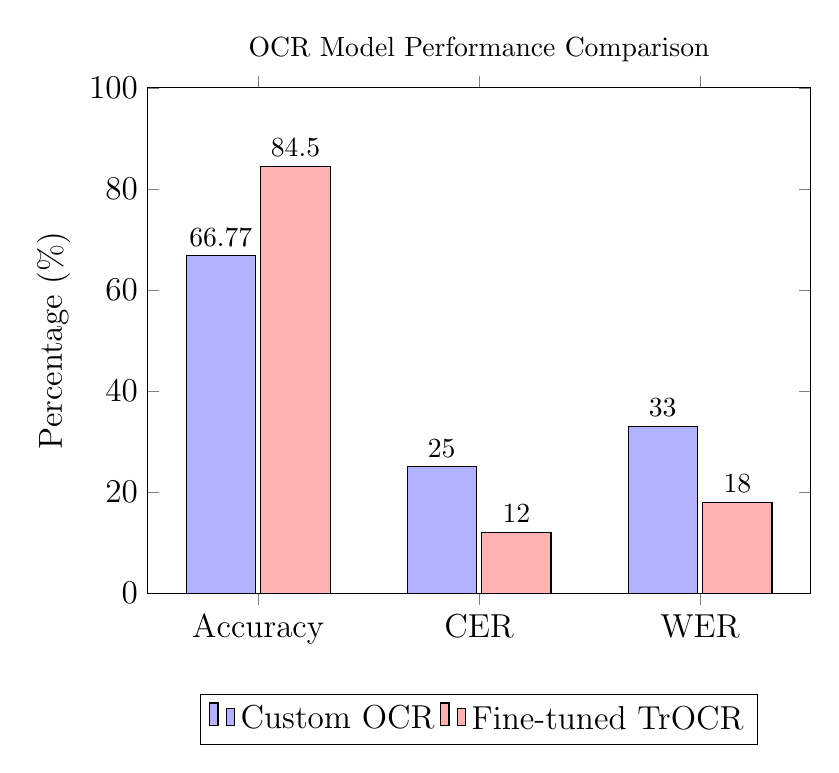
\begin{tikzpicture}
        \begin{axis}[
            ybar,
            enlarge x limits=0.25,
            legend style={at={(0.5,-0.2)},
              anchor=north,legend columns=-1},
            ylabel={Percentage (\%)},
            symbolic x coords={Accuracy, CER, WER},
            xtick=data,
            nodes near coords,
            nodes near coords align={vertical},
            ymin=0, ymax=100,
            bar width=25pt,
            width=10cm,
            height=8cm,
            title={OCR Model Performance Comparison},
            % Ensure 12pt style for labels
            label style={font=\large},
            tick label style={font=\large},
            legend style={font=\large}
        ]
            % Custom CRNN Data
            % CER (0.25 -> 25) and WER (0.33 -> 33)
            \addplot [fill=blue!30] coordinates {(Accuracy,66.77) (CER,25) (WER,33)};
            
            % Fine-tuned TrOCR Data
            % CER (0.12 -> 12) and WER (0.18 -> 18)
            \addplot [fill=red!30] coordinates {(Accuracy,84.50) (CER,12) (WER,18)};
            
            \legend{Custom OCR, Fine-tuned TrOCR}
        \end{axis}
    \end{tikzpicture}
    \caption{Performance metrics comparison, in percentage}
    \label{fig:ocr-bar-chart}
\end{figure}

\cref{table:ocr-comparison} summarizes the performance of both \gls{ocr} models, and \cref{fig:ocr-bar-chart} provides a visual comparison. The fine-tuned TrOCR model outperforms the custom \gls{crnn} across all metrics despite requiring only 3 training epochs compared to 27 (tested on the test split of the CGHD dataset). The \gls{cer} reduction from 0.25 to 0.12 indicates that TrOCR makes half as many character-level errors, directly improving the accuracy of extracted component values. It is noted that the custom \gls{crnn}'s lower accuracy (66.77\%) was partly attributed to data corruption during preprocessing. Regardless, the architectural advantages of the Transformer-based approach make TrOCR the superior choice for this pipeline. However, the inference speed of TrOCR has found to be considerably slower than the custom OCR model. This implies there is inherently a trade-off between accuracy and inference speed when choosing between the custom OCR and TrOCR models for this project. Keeping this in mind, both models are retained in the codebase and can be switched based on user preference.

\section{\gls{ocr} Demonstration}

Two randomly picked images from the dataset are shown below after passing through the detection (\gls{yolo}v7) and recognition (\gls{ocr}) models.

\begin{figure}[H]
    \centering
    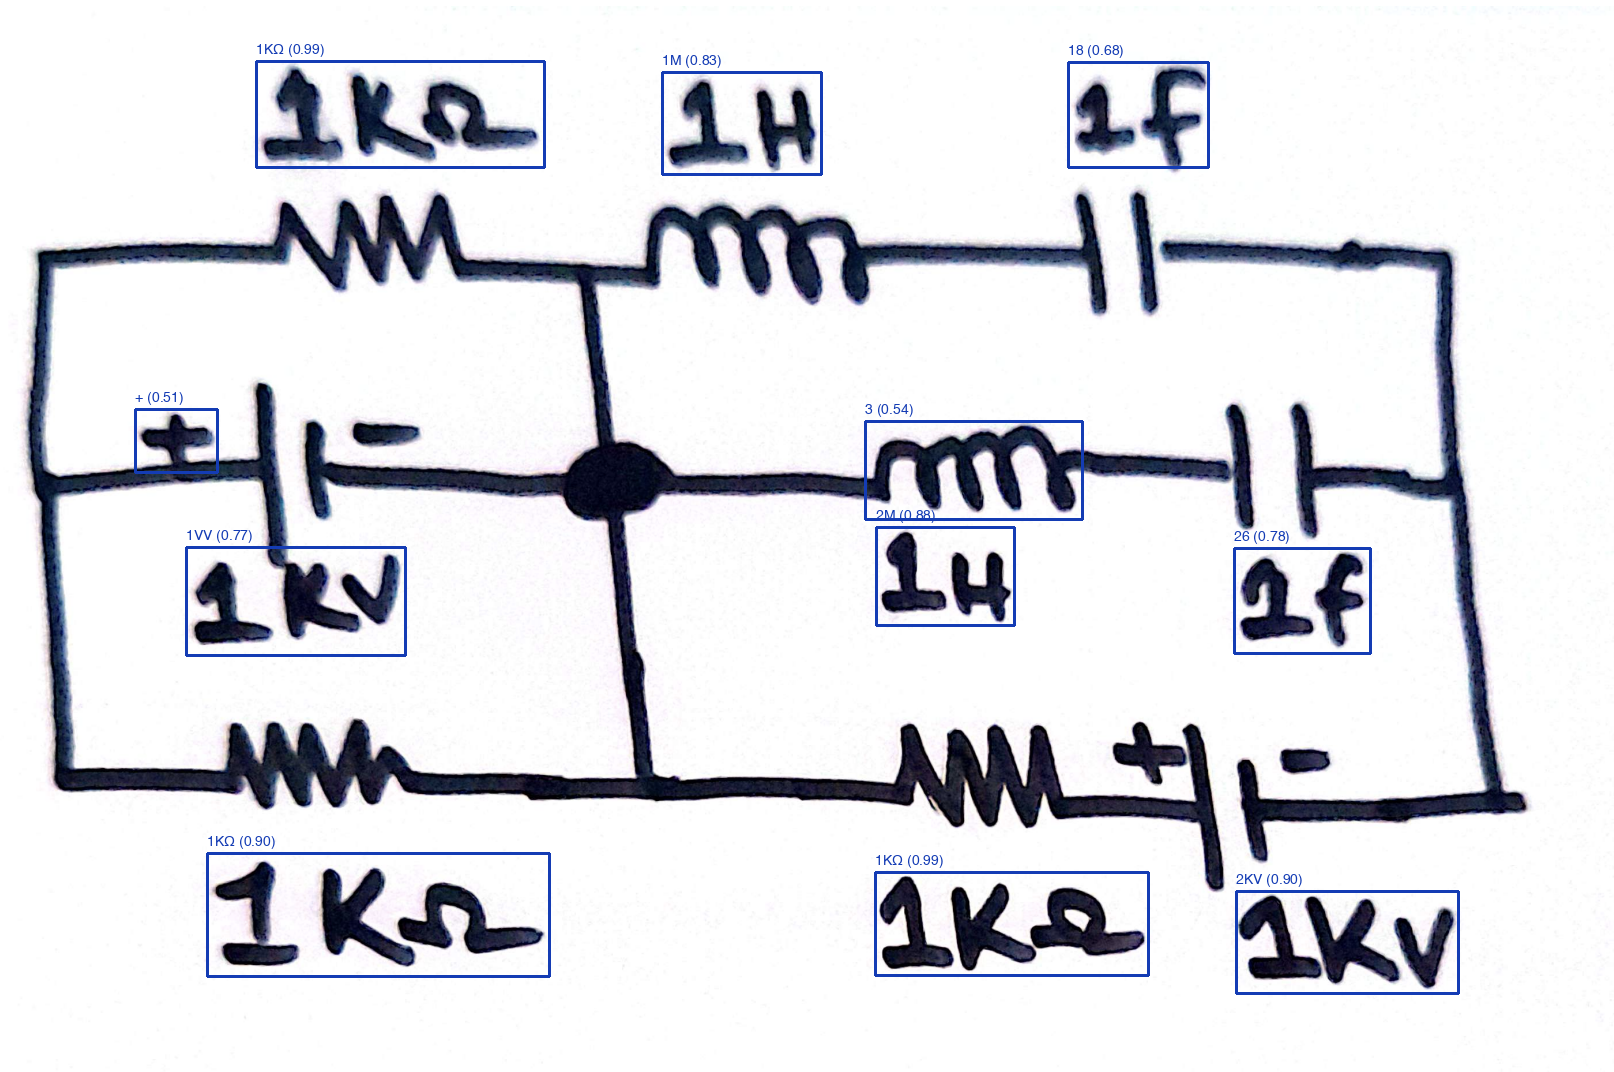
\includegraphics[width=\textwidth]{src/images/figures/custom_ocr_result1.png}
    \caption{Text Detection and Recognition using Custom OCR(i)}
    \label{fig:custom-ocr-result-1}
\end{figure}

\begin{figure}[H]
    \centering
    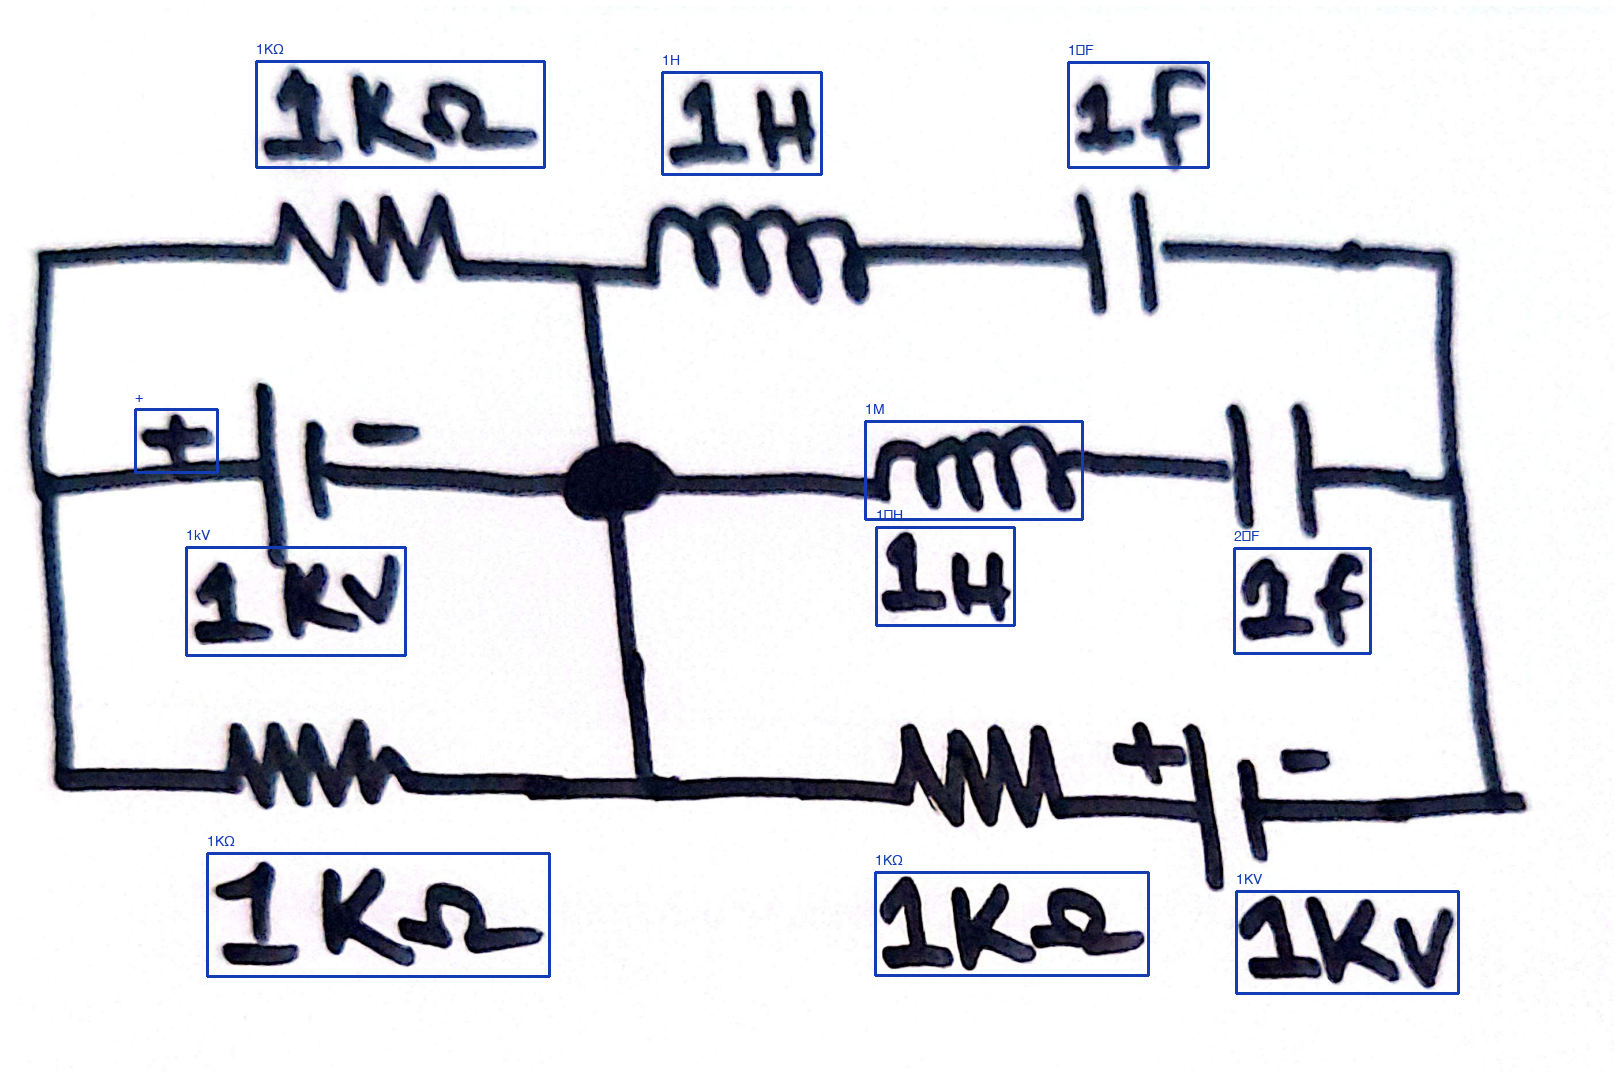
\includegraphics[width=\textwidth]{src/images/figures/trocr_result1.png}
    \caption{Text Detection and Recognition using TrOCR(i)}
    \label{fig:trocr-result-1}
\end{figure}

\begin{figure}[H]
    \centering
    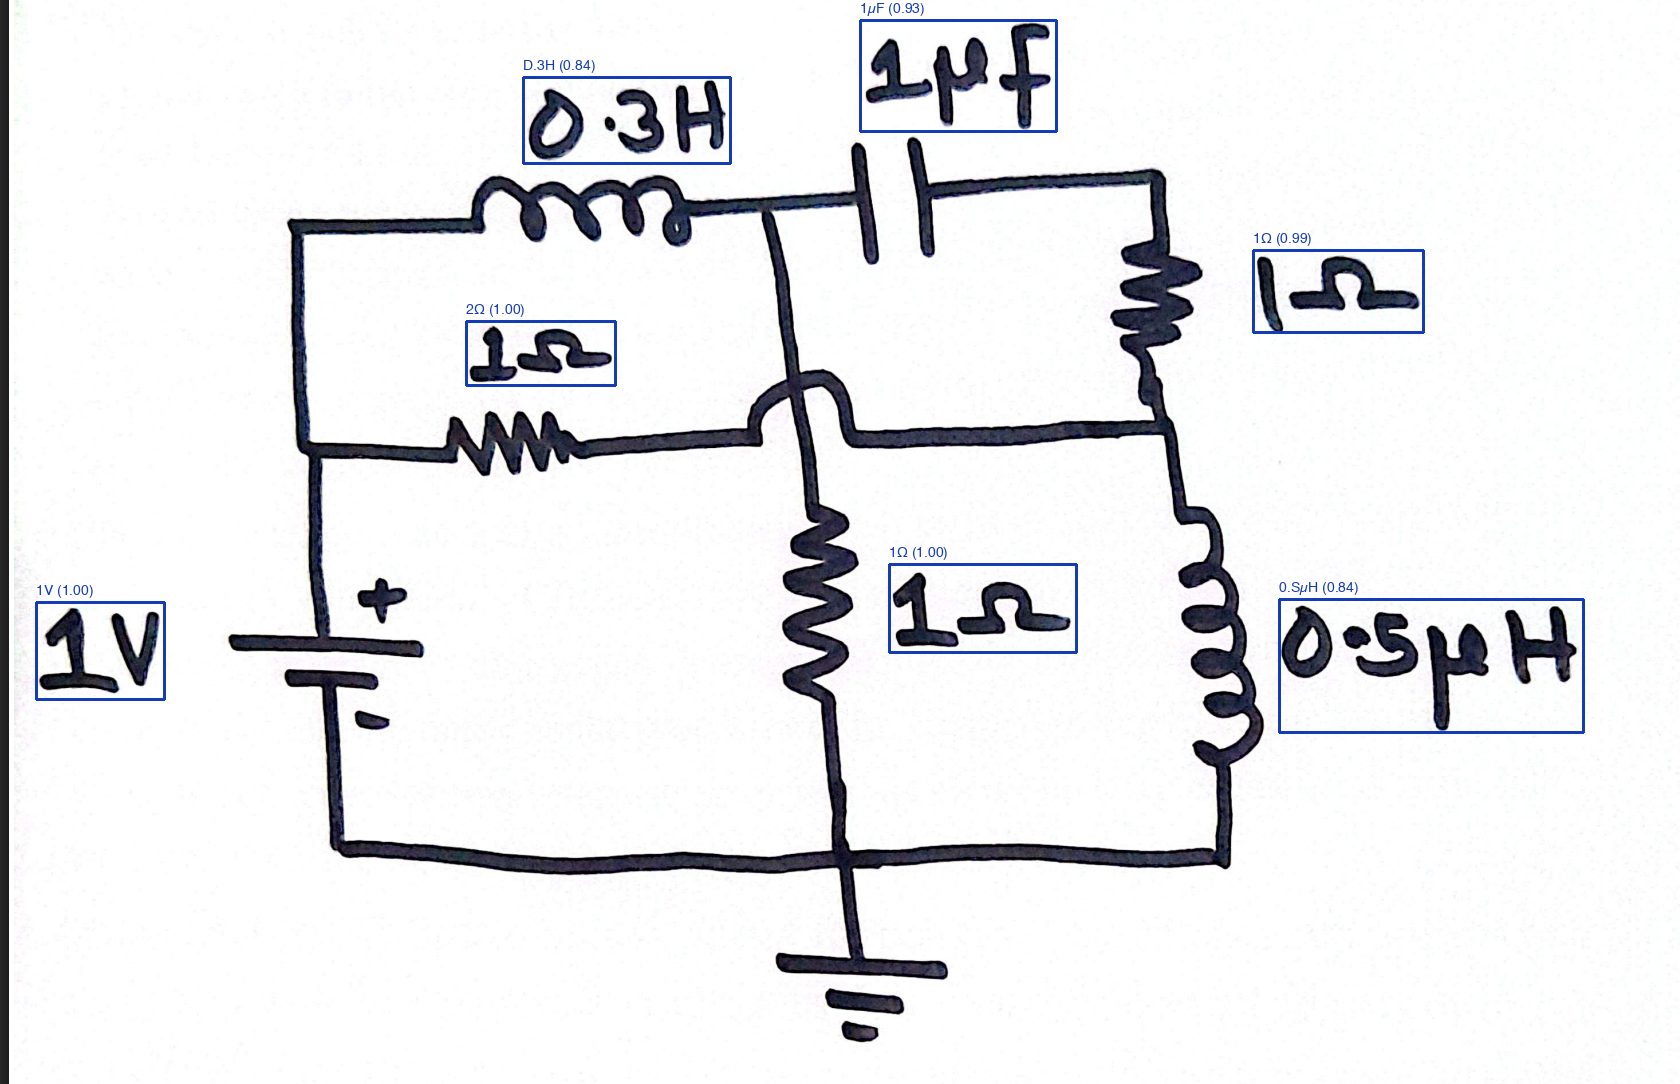
\includegraphics[width=\textwidth]{src/images/figures/custom_ocr_result2.png}
    \caption{Text Detection and Recognition using Custom OCR(ii)}
    \label{fig:custom-ocr-result-2}
\end{figure}

\begin{figure}[H]
    \centering
    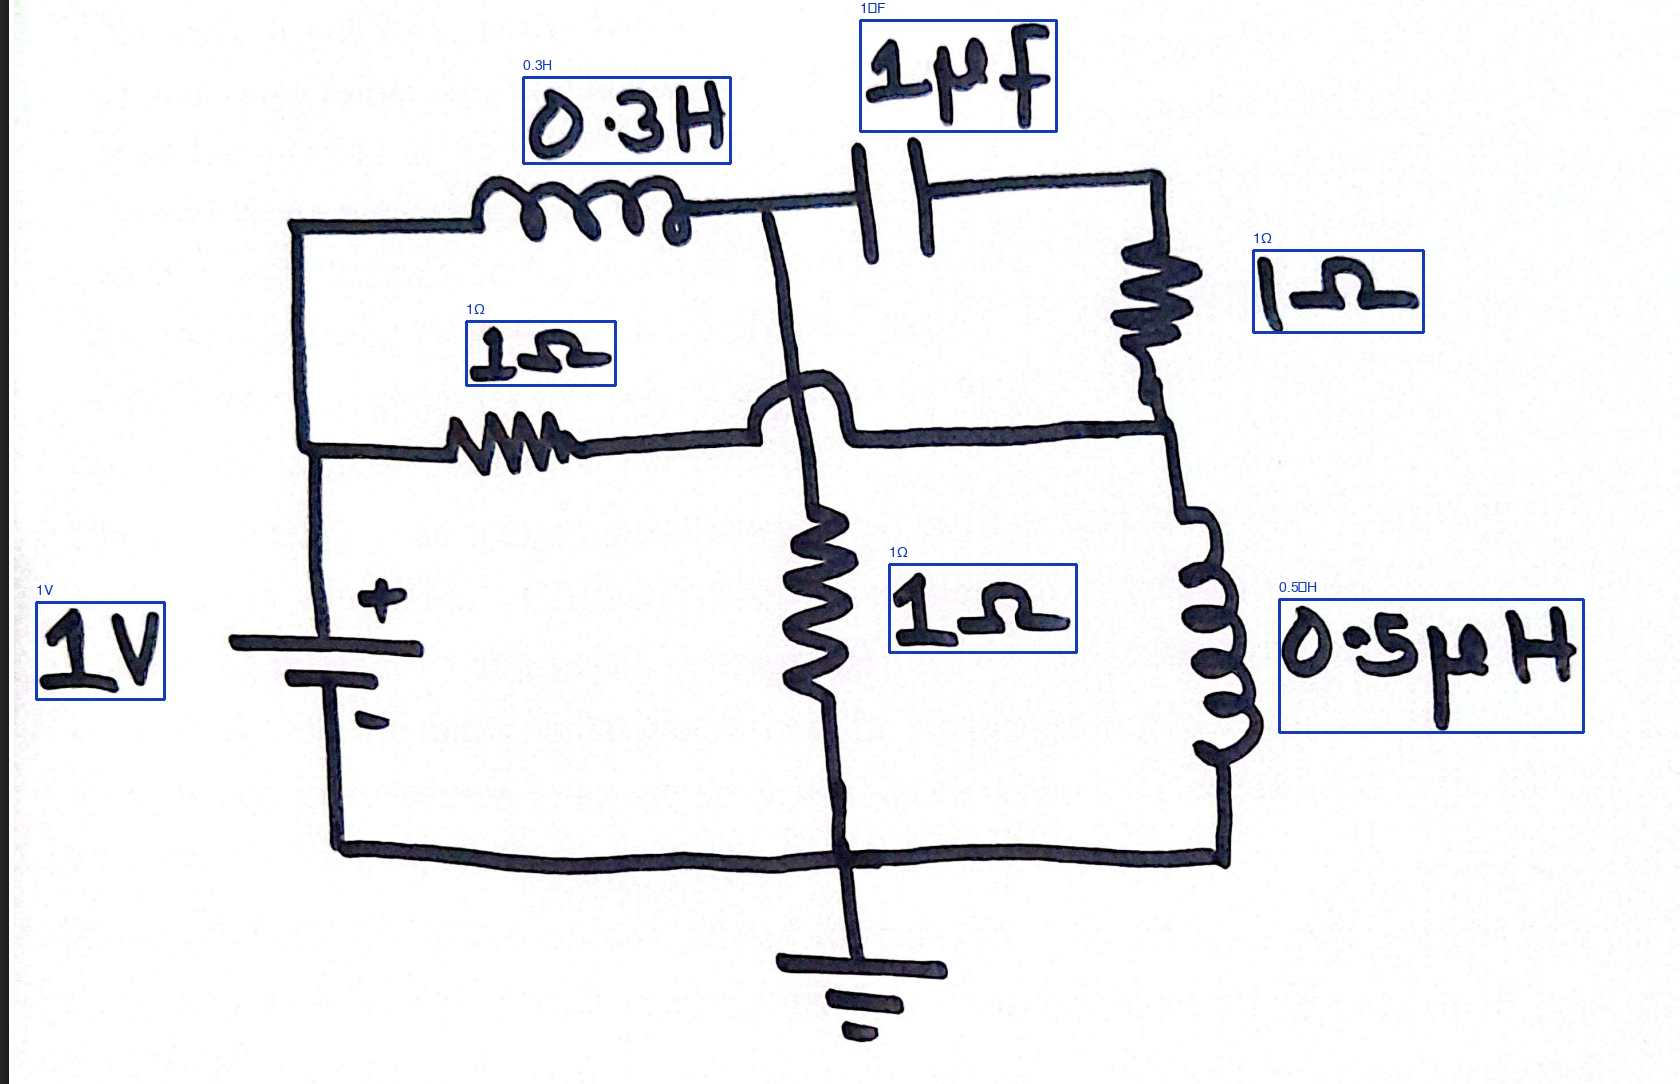
\includegraphics[width=\textwidth]{src/images/figures/trocr_result2.png}
    \caption{Text Detection and Recognition using TrOCR(ii)}
    \label{fig:trocr-result-2}
\end{figure}

\cref{fig:custom-ocr-result-1} and \cref{fig:custom-ocr-result-2} show the results of the custom OCR model on two random test images. The model successfully detects text regions and extracts component values, albeit with many errors. \cref{fig:trocr-result-1} and \cref{fig:trocr-result-2} show the results of the fine-tuned TrOCR model which clearly shows better performance recognizing more component values accurately.

\section{Junction-Based Wire Detection}

\begin{figure}[H]
    \centering
    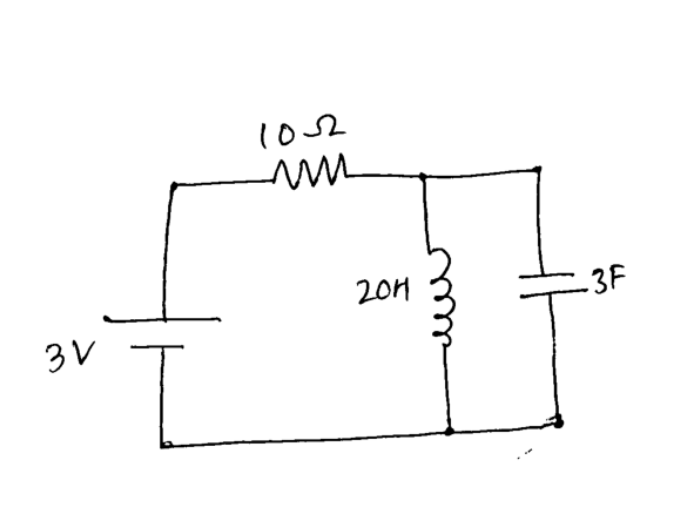
\includegraphics[width=\textwidth]{src/images/figures/otsu_thresholding.png}
    \caption{Otsu's Global Thresholding}
    \label{fig:otsu-thresholding}
\end{figure}

In the junction-based wire detection pipeline, the uploaded image is first binarized using Otsu's Thresholding as shown in \cref{fig:otsu-thresholding}. This binarized image is skeletonized i.e., the width of every line is thinned down to a single pixel and the component bounding boxes are superimposed into this skeletonized circuit as shown in \cref{fig:bbox-overlay}.

\begin{figure}[H]
    \centering
    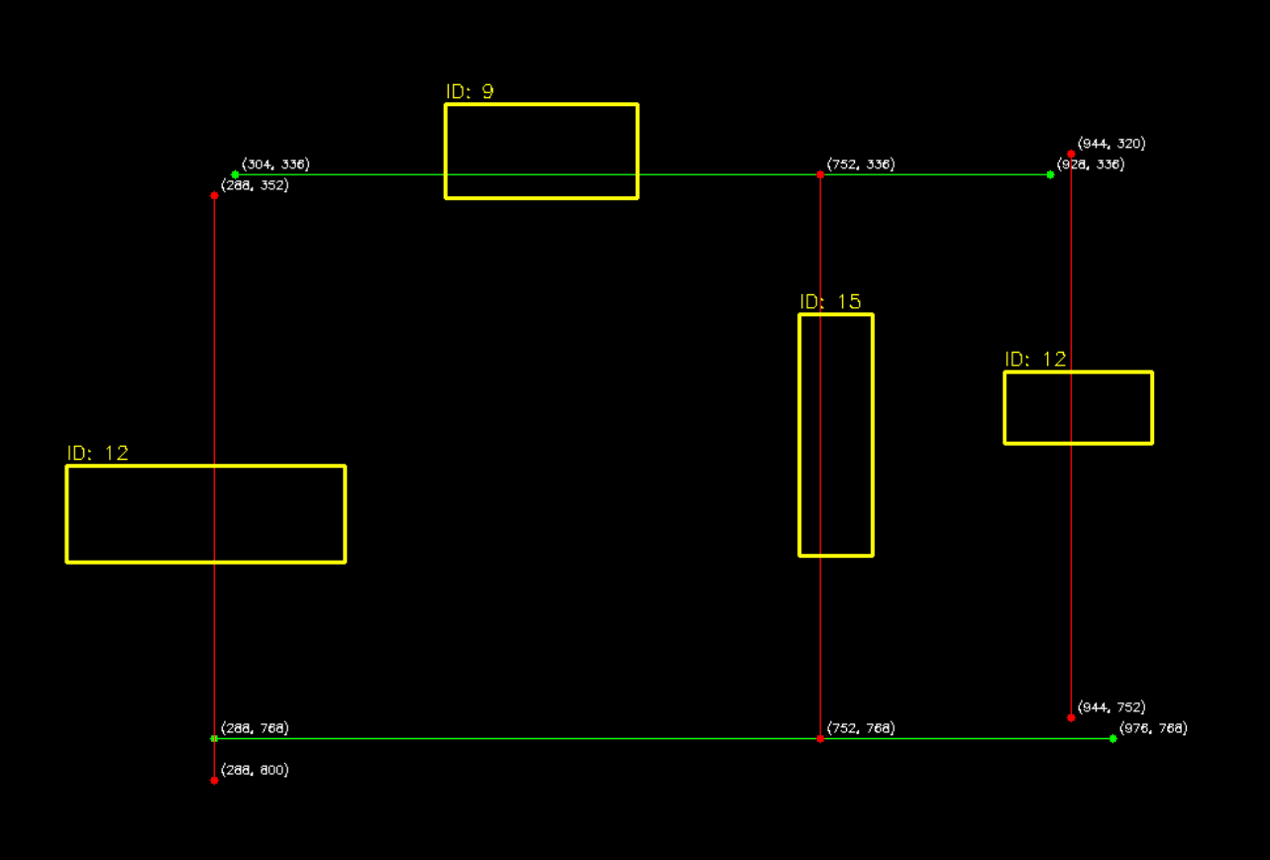
\includegraphics[width=\textwidth]{src/images/figures/bounding_box_overlay.png}
    \caption{Bounding Box Overlay}
    \label{fig:bbox-overlay}
\end{figure}

\section{Visualization of Line Detection via Path Finding}

\subsection{Skeletonized Image with Detected Endpoints}

\begin{figure}[H]
    \centering
    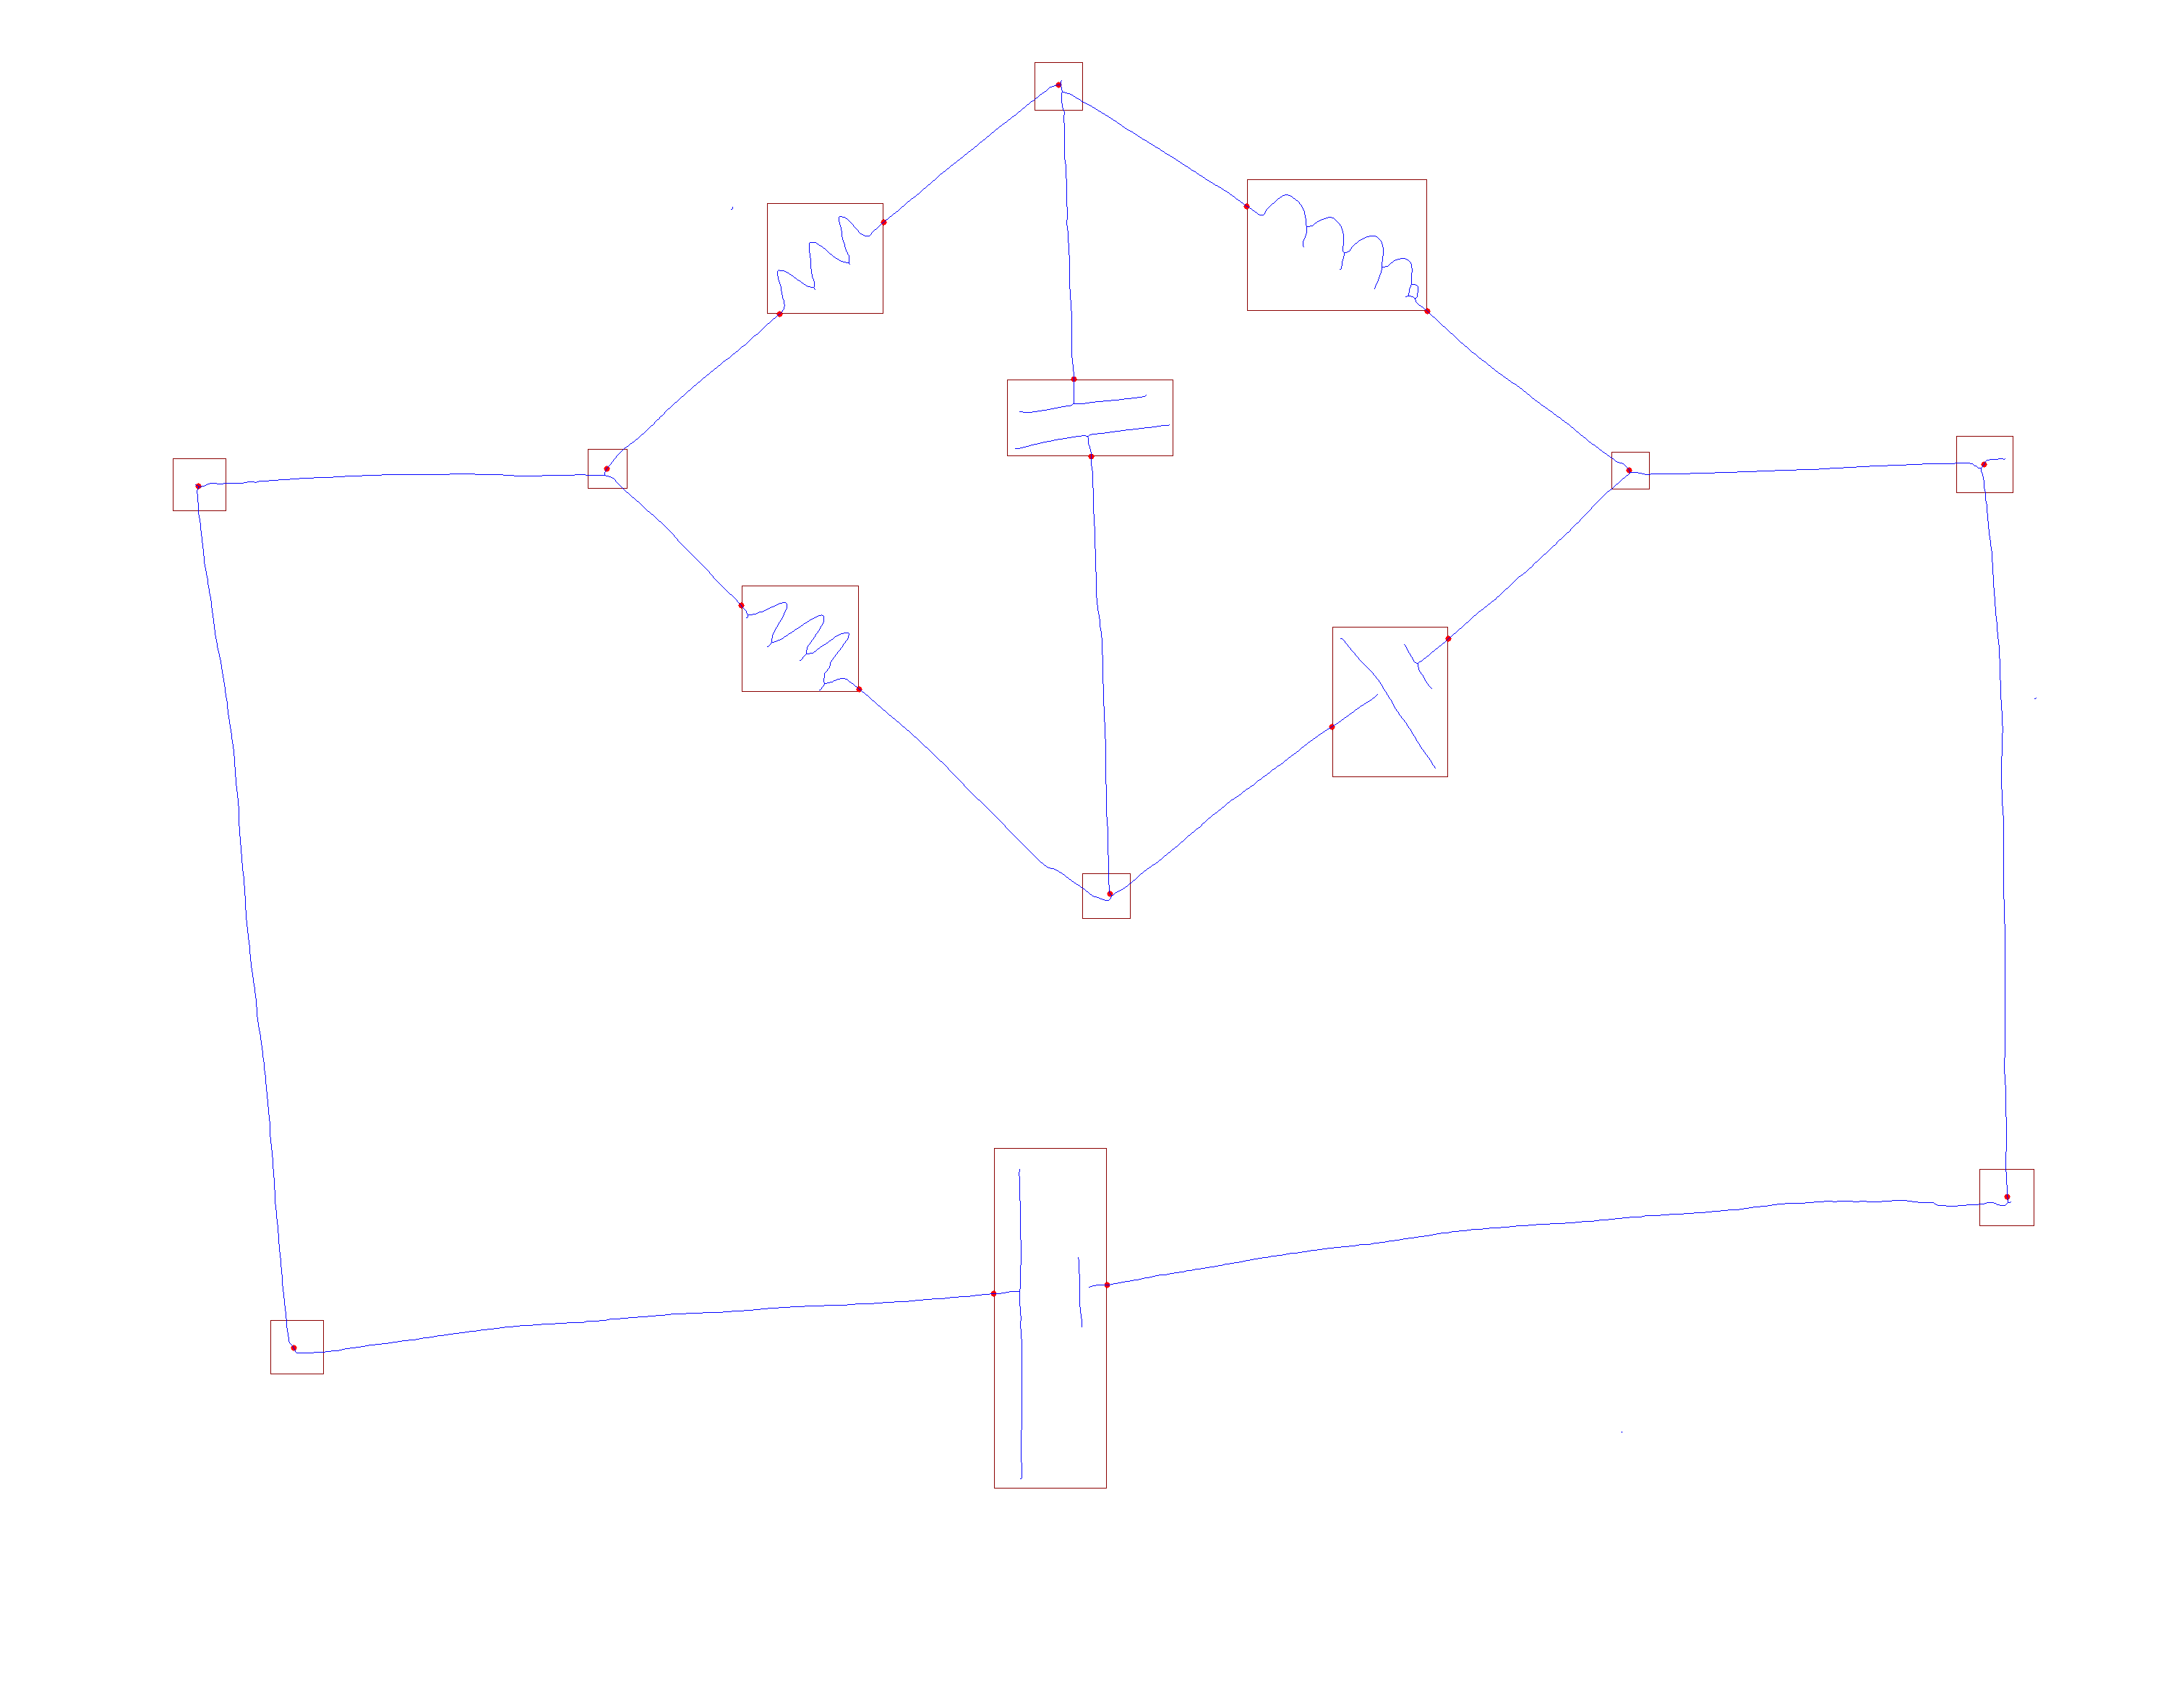
\includegraphics[width=0.8\textwidth]{src/images/figures/skeleton_with_endpoints.png}
    \caption{Skeletonized Image with Detected Endpoints}
    \label{fig:skeleton_endpoints}
\end{figure}

Line detection via path finding also requires skeletonization. \cref{fig:skeleton_endpoints} shows the overlay of the bounding boxes in the skeletonized circuit. The blue rectangles signify the bounding boxes as given by the YOLO model, and the blue dots signify the endpoints (used as nodes for BFS).

\subsection{Adjacency Graph Visualization}

\begin{figure}[H]
    \centering
    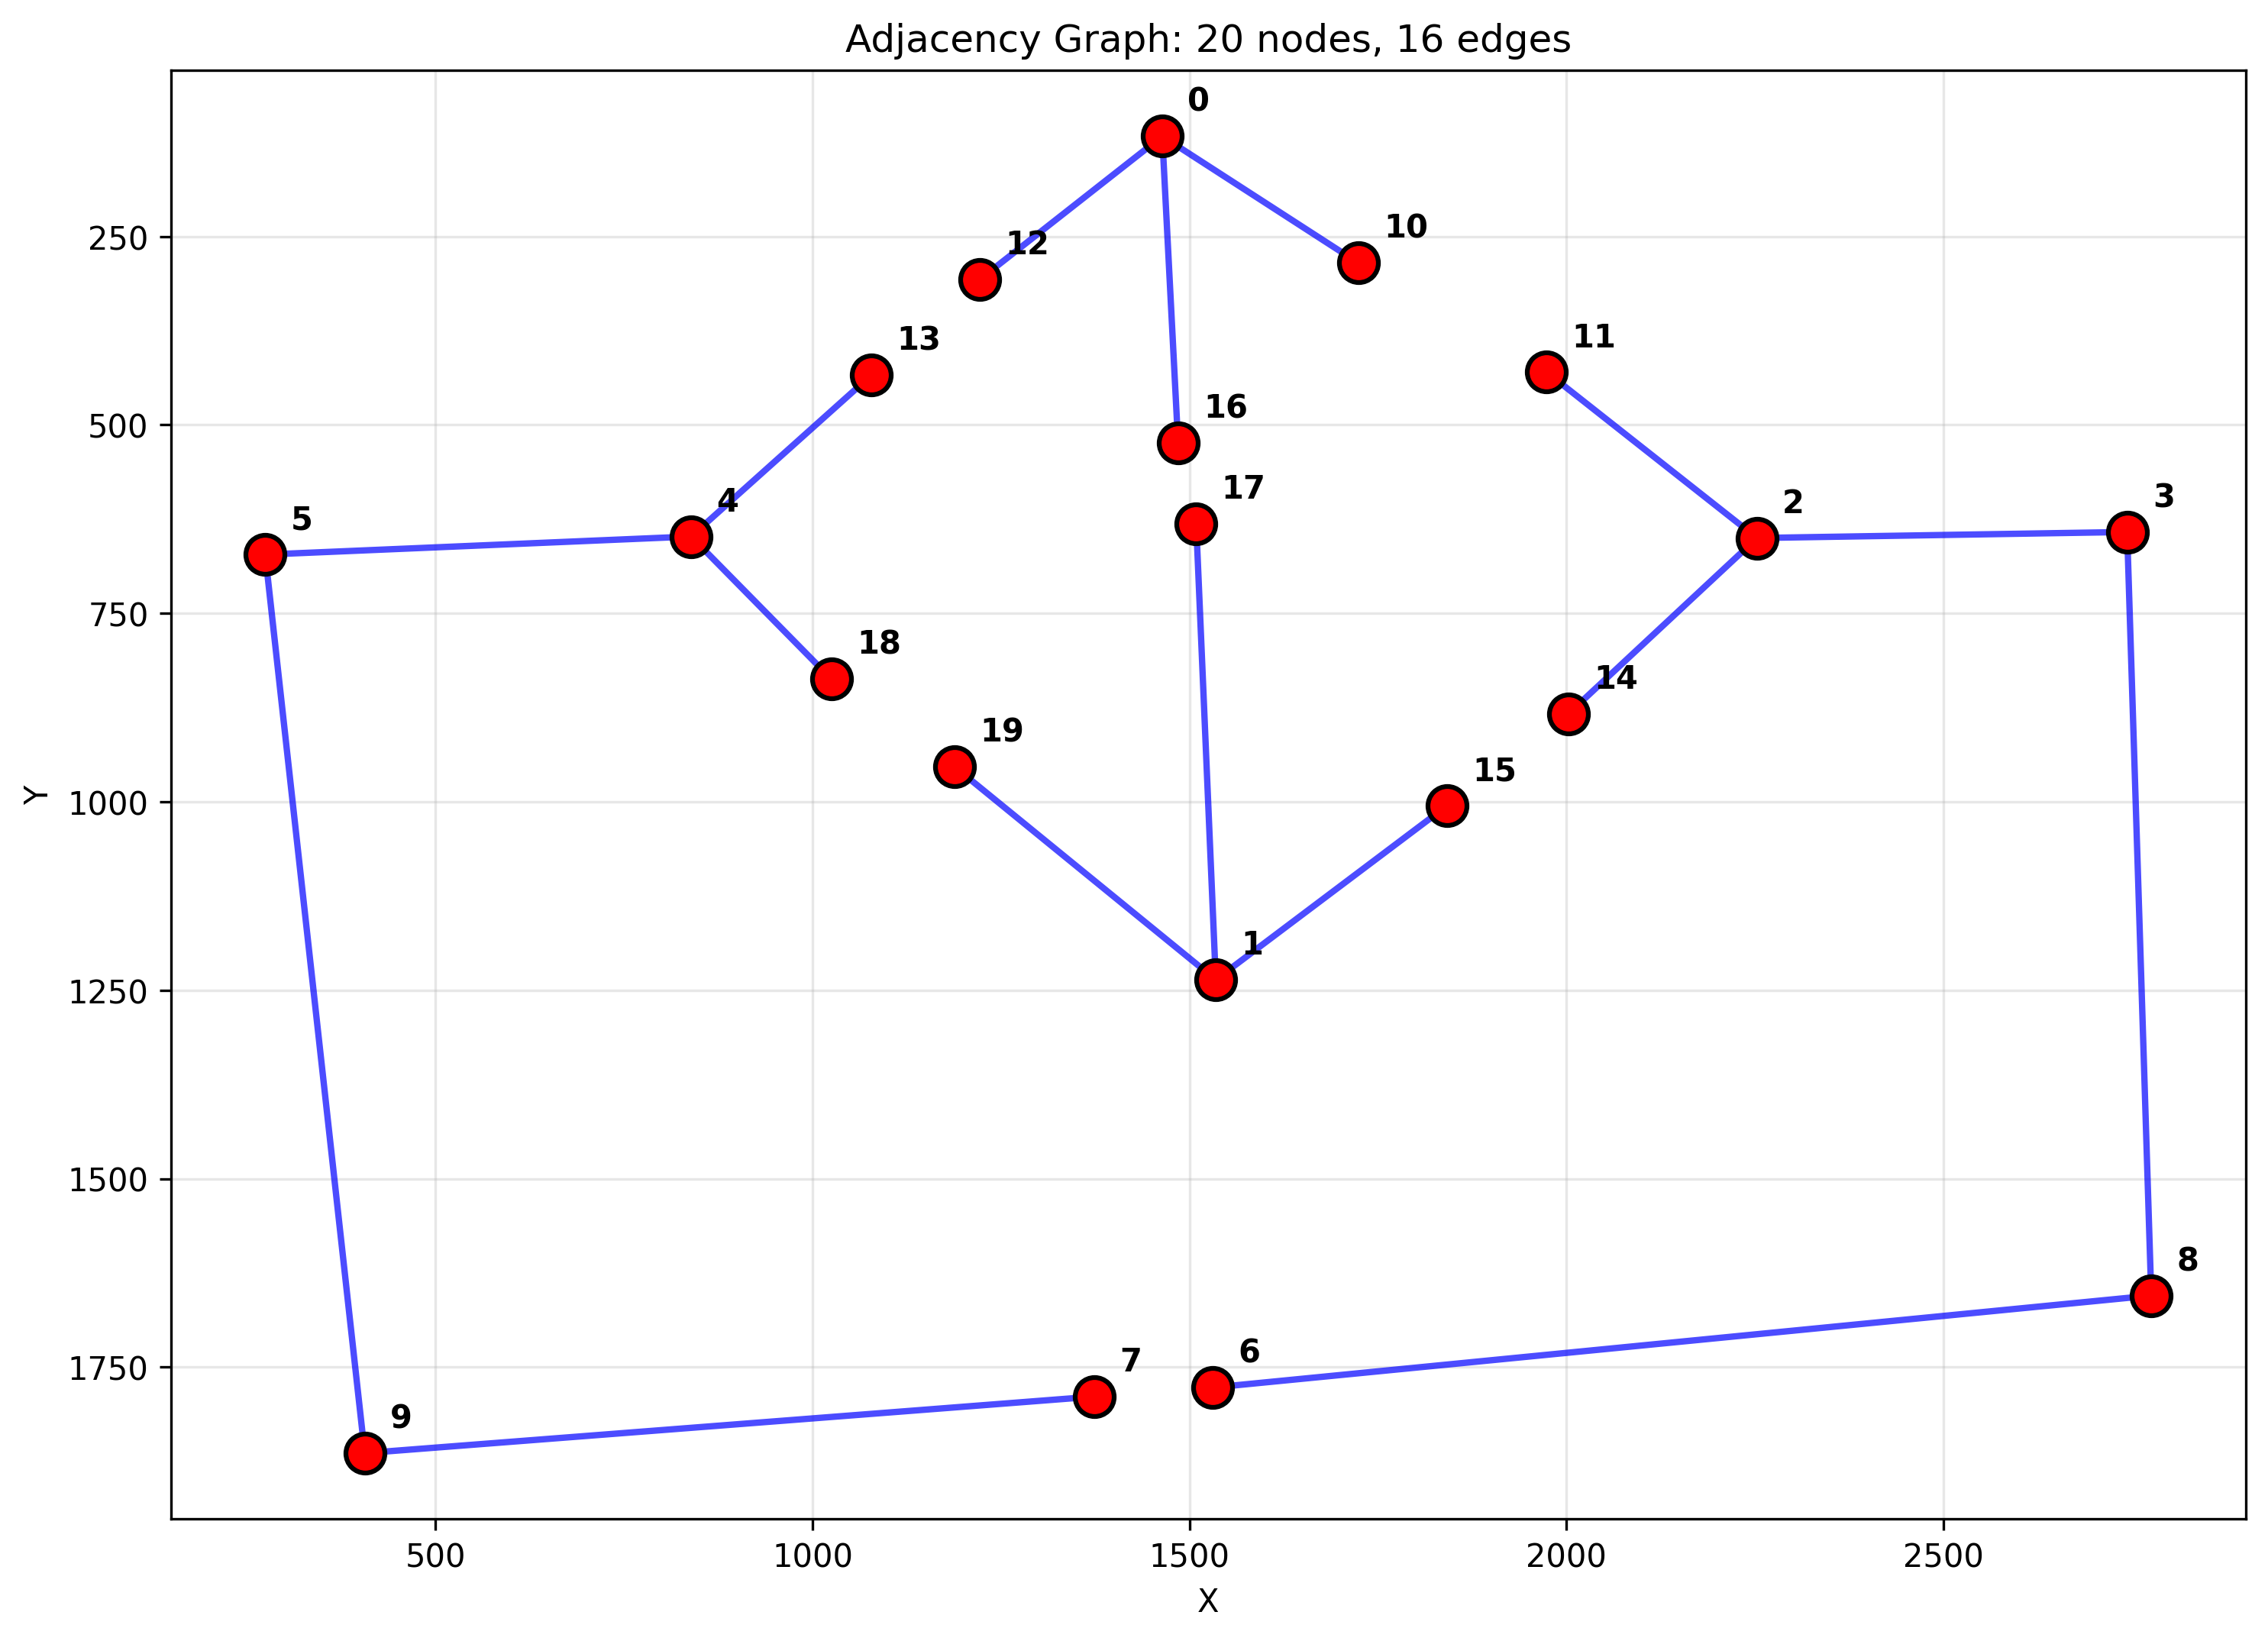
\includegraphics[width=0.7\textwidth]{src/images/figures/adjacency_graph.png}
    \caption{Adjacency graph constructed using Multi-Head BFS algorithm}
    \label{fig:adjacency_graph}
\end{figure}

\cref{fig:adjacency_graph} shows the adjacency graph produced by the Multi-Head BFS algorithm with blue lines representing the edges between the red nodes (the self edges have been pruned). The empty spaces between some nodes are where the circuit components were situated in the sketch and will later be added in the digital schematic.

\section{Combined Overlay of YOLOv7, TrOCR, and Line Detection Results}

\begin{figure}[H]
    \centering
    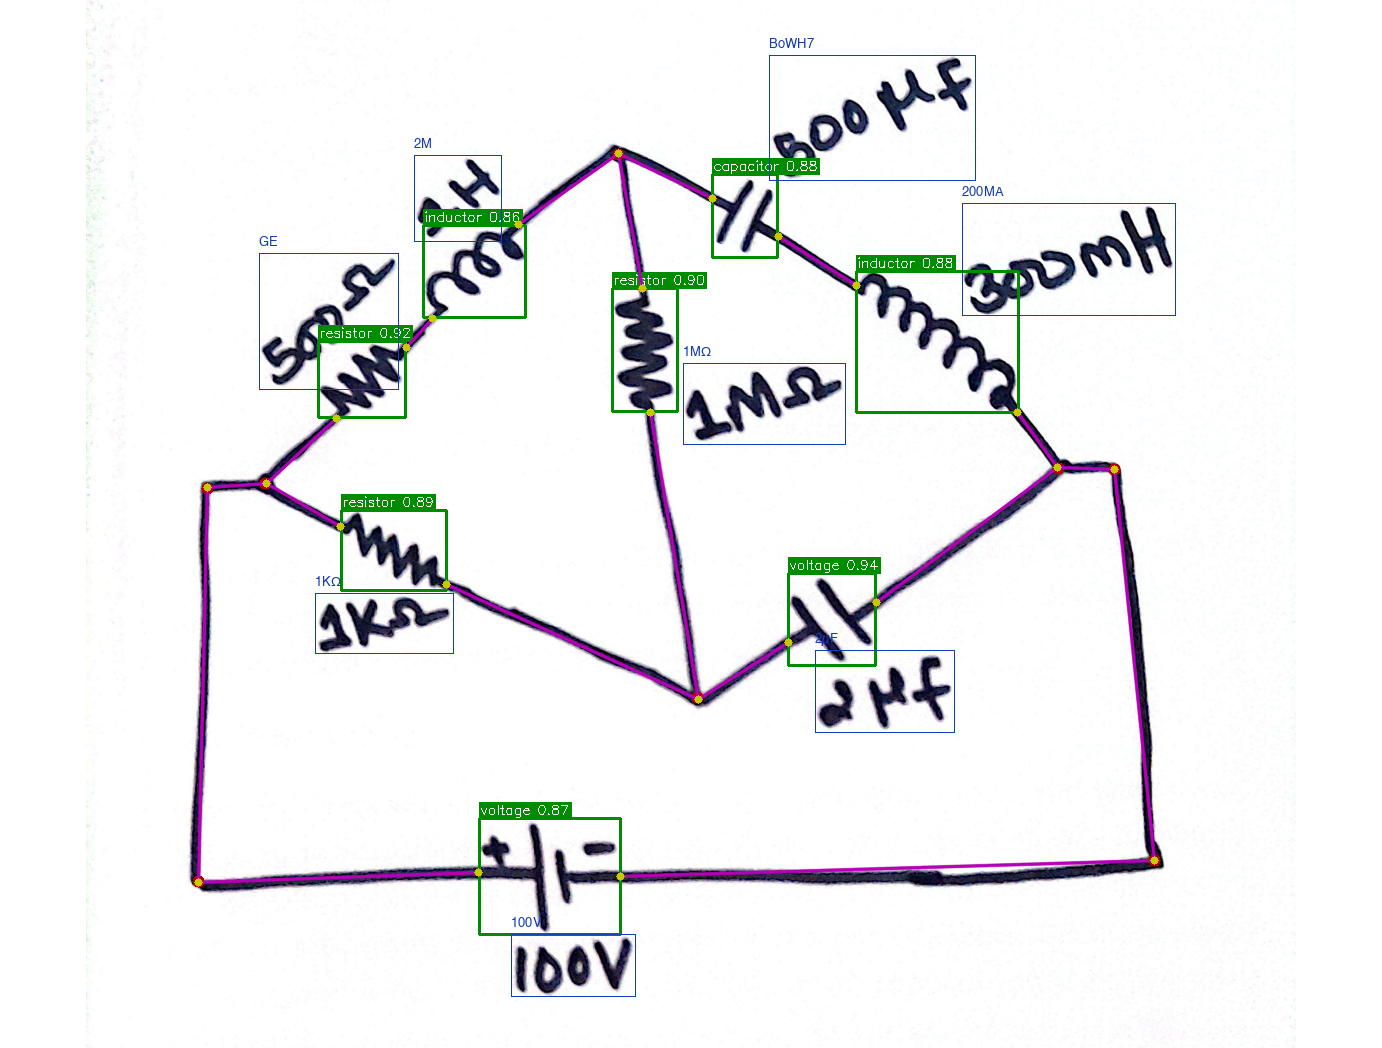
\includegraphics[width=0.7\textwidth]{src/images/figures/combined_overlay.png}
    \caption{Combined Results of YOLOv7, TrOCR, and Line Detection}
    \label{fig:combined_overlay}
\end{figure}

\cref{fig:combined_overlay} shows the combined effect of the result from component detection (green bounding boxes), text recognition (blue rectangles with text annotations), and line detection (red wire tracings) overlaid in a Whetstone bridge circuit. 

\section{Frontend Visualization}

\begin{figure}[H]
    \centering
    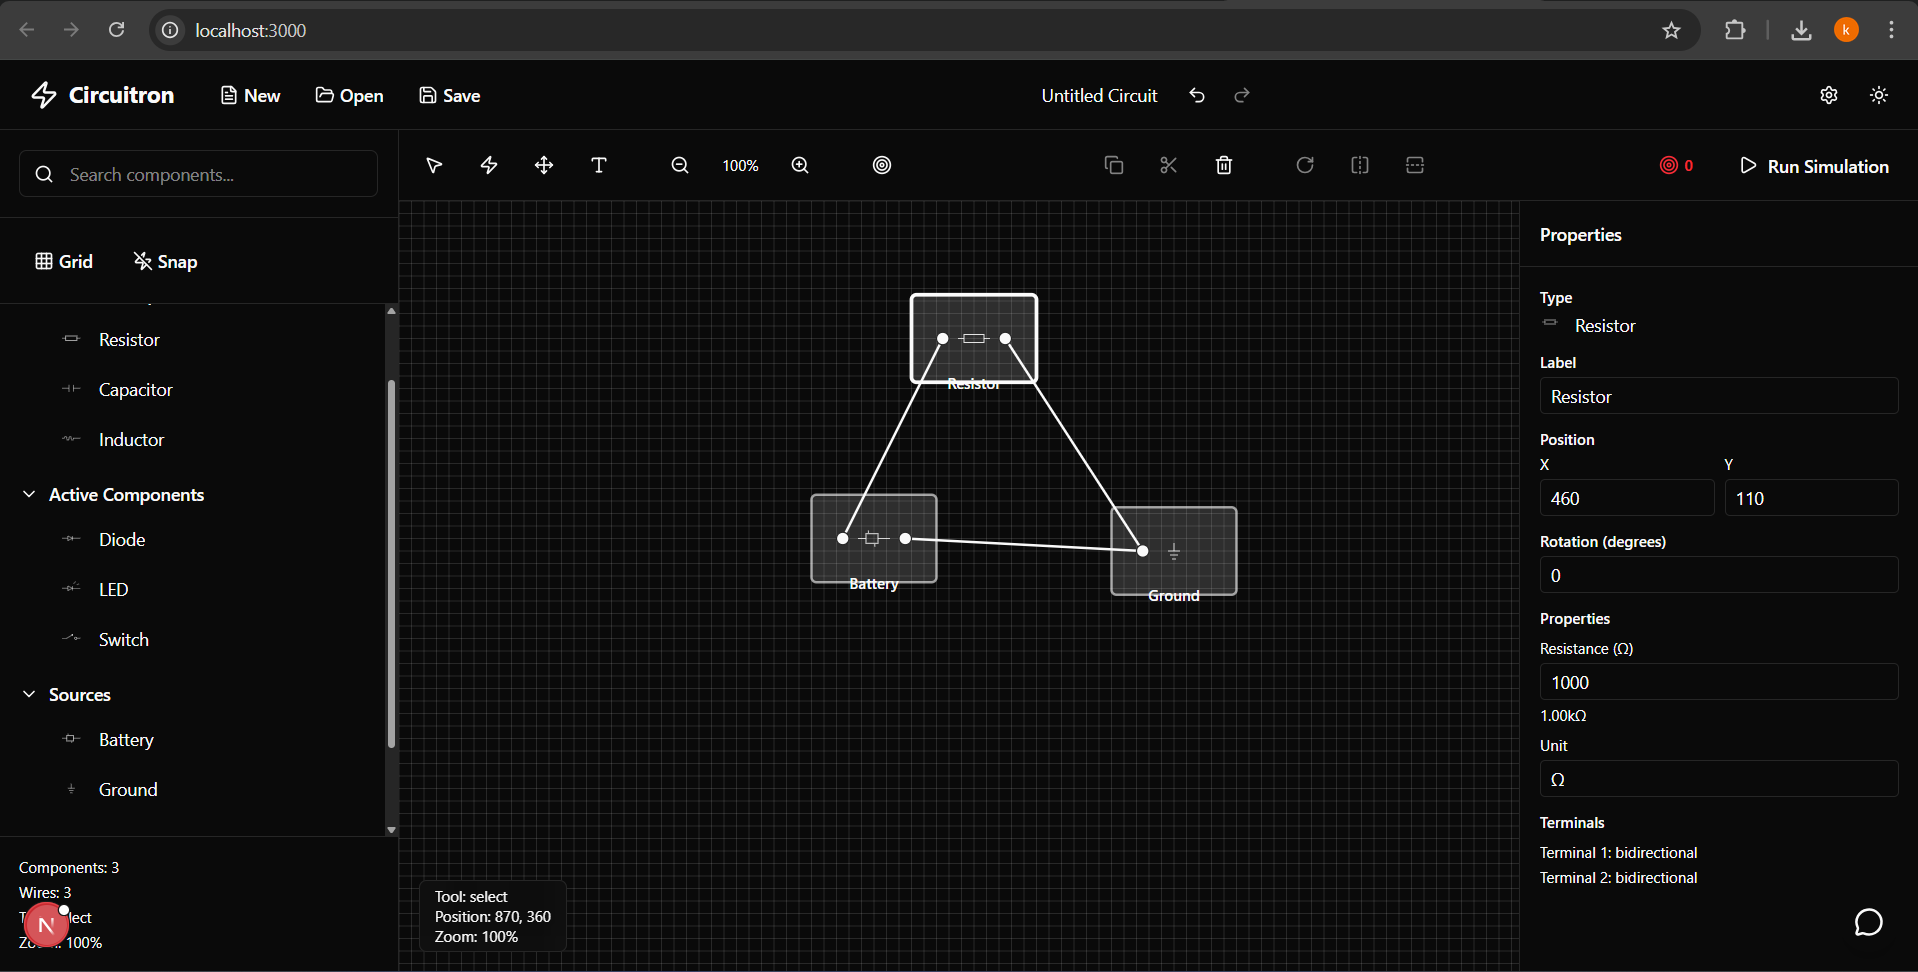
\includegraphics[width=\textwidth]{src/images/figures/frontend_circuit.png}
    \caption{Digitally Drawn Circuit (Color Inverted)}
    \label{fig:digital-circuit-editor}
\end{figure}

\begin{figure}[H]
    \centering
    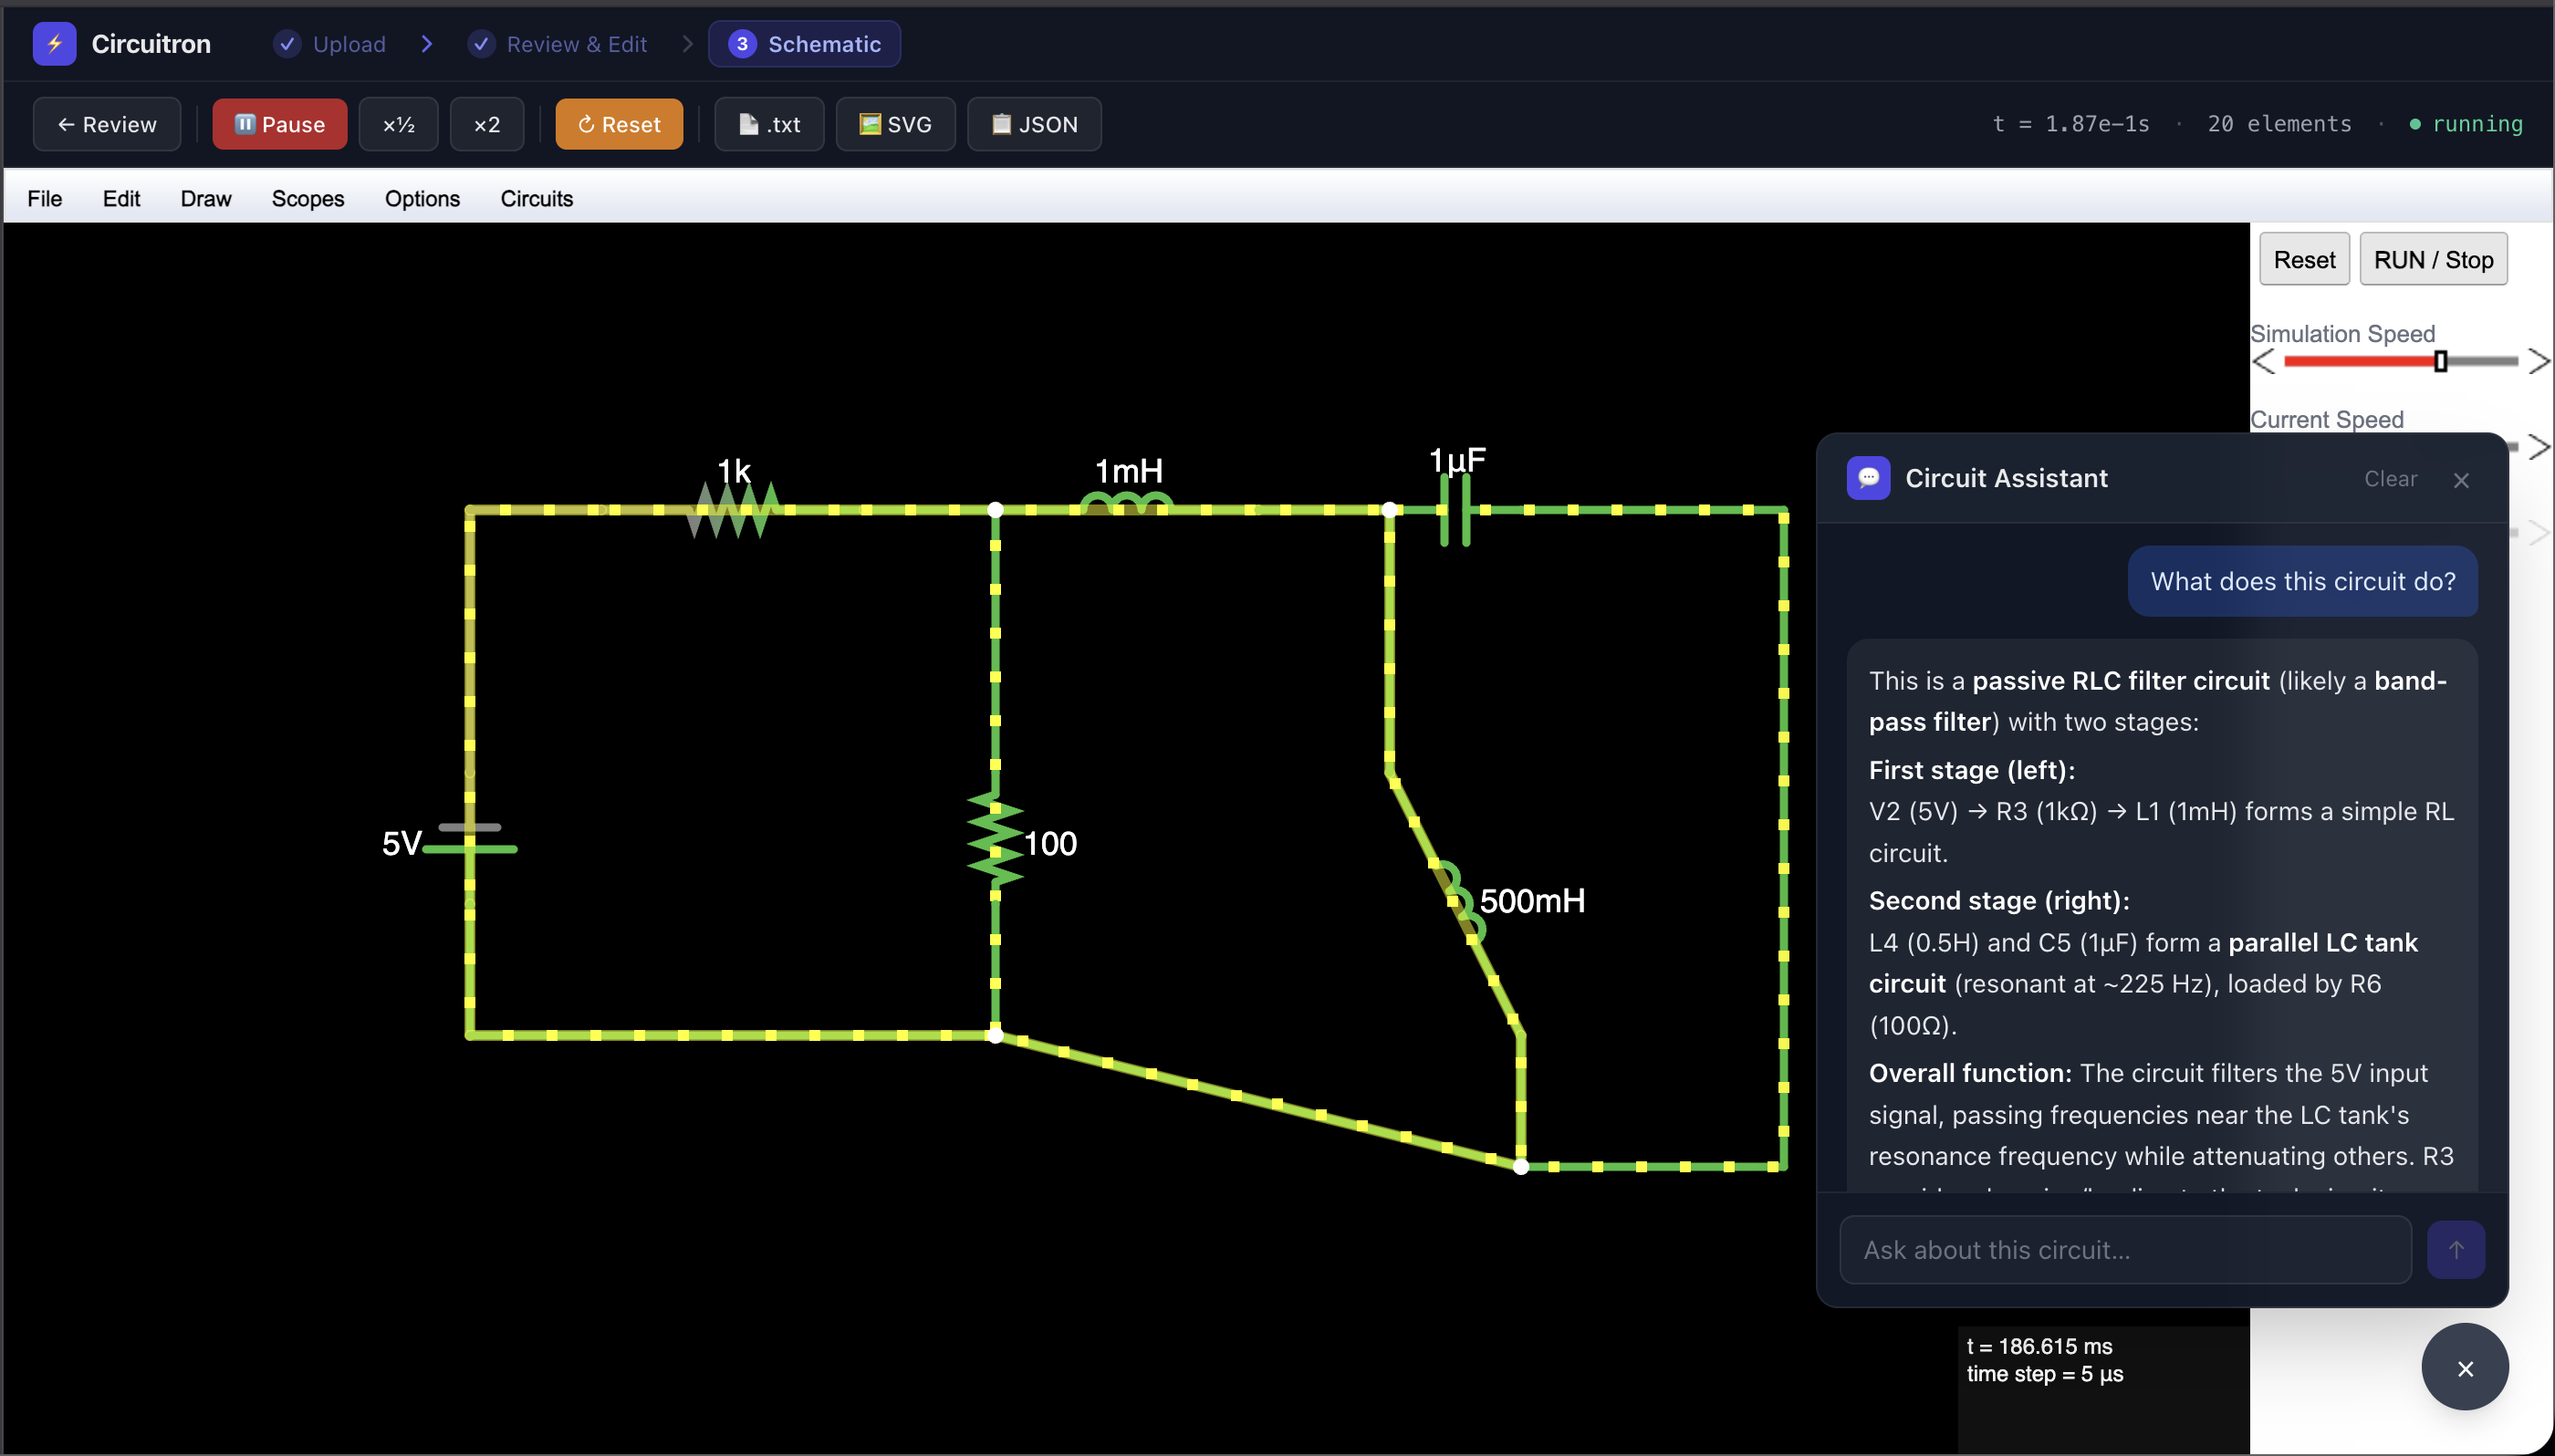
\includegraphics[width=\textwidth]{src/images/figures/frontend_screenshot.png}
    \caption{Fullscreen Capture of the Frontend}
    \label{fig:frontend-screenshot}
\end{figure}

Figure \ref{fig:digital-circuit-editor} shows the digitized version of the hand-drawn circuit fed into the system. This is just the automatically generated schematic before any manual intervention. Figure \ref{fig:frontend-screenshot} shows the full-screen capture of the frontend of the system with a circuit diagram, options to modify this diagram in the menu bar, simulation setting towards the right, and also the LLM-powered Q&A feature. Measurement probes let users monitor signals in real time while the system automatically computes peak-to-peak swing and \gls{rms} values alongside maxima and minima. Simulation data and plots can also be exported in standard formats for offline review or inclusion in documentation. 



